% Options for packages loaded elsewhere
\PassOptionsToPackage{unicode}{hyperref}
\PassOptionsToPackage{hyphens}{url}
%
\documentclass[
]{article}
\usepackage{amsmath,amssymb}
\usepackage{iftex}
\ifPDFTeX
  \usepackage[T1]{fontenc}
  \usepackage[utf8]{inputenc}
  \usepackage{textcomp} % provide euro and other symbols
\else % if luatex or xetex
  \usepackage{unicode-math} % this also loads fontspec
  \defaultfontfeatures{Scale=MatchLowercase}
  \defaultfontfeatures[\rmfamily]{Ligatures=TeX,Scale=1}
\fi
\usepackage{lmodern}
\ifPDFTeX\else
  % xetex/luatex font selection
\fi
% Use upquote if available, for straight quotes in verbatim environments
\IfFileExists{upquote.sty}{\usepackage{upquote}}{}
\IfFileExists{microtype.sty}{% use microtype if available
  \usepackage[]{microtype}
  \UseMicrotypeSet[protrusion]{basicmath} % disable protrusion for tt fonts
}{}
\makeatletter
\@ifundefined{KOMAClassName}{% if non-KOMA class
  \IfFileExists{parskip.sty}{%
    \usepackage{parskip}
  }{% else
    \setlength{\parindent}{0pt}
    \setlength{\parskip}{6pt plus 2pt minus 1pt}}
}{% if KOMA class
  \KOMAoptions{parskip=half}}
\makeatother
\usepackage{xcolor}
\usepackage[margin=1in]{geometry}
\usepackage{color}
\usepackage{fancyvrb}
\newcommand{\VerbBar}{|}
\newcommand{\VERB}{\Verb[commandchars=\\\{\}]}
\DefineVerbatimEnvironment{Highlighting}{Verbatim}{commandchars=\\\{\}}
% Add ',fontsize=\small' for more characters per line
\usepackage{framed}
\definecolor{shadecolor}{RGB}{248,248,248}
\newenvironment{Shaded}{\begin{snugshade}}{\end{snugshade}}
\newcommand{\AlertTok}[1]{\textcolor[rgb]{0.94,0.16,0.16}{#1}}
\newcommand{\AnnotationTok}[1]{\textcolor[rgb]{0.56,0.35,0.01}{\textbf{\textit{#1}}}}
\newcommand{\AttributeTok}[1]{\textcolor[rgb]{0.13,0.29,0.53}{#1}}
\newcommand{\BaseNTok}[1]{\textcolor[rgb]{0.00,0.00,0.81}{#1}}
\newcommand{\BuiltInTok}[1]{#1}
\newcommand{\CharTok}[1]{\textcolor[rgb]{0.31,0.60,0.02}{#1}}
\newcommand{\CommentTok}[1]{\textcolor[rgb]{0.56,0.35,0.01}{\textit{#1}}}
\newcommand{\CommentVarTok}[1]{\textcolor[rgb]{0.56,0.35,0.01}{\textbf{\textit{#1}}}}
\newcommand{\ConstantTok}[1]{\textcolor[rgb]{0.56,0.35,0.01}{#1}}
\newcommand{\ControlFlowTok}[1]{\textcolor[rgb]{0.13,0.29,0.53}{\textbf{#1}}}
\newcommand{\DataTypeTok}[1]{\textcolor[rgb]{0.13,0.29,0.53}{#1}}
\newcommand{\DecValTok}[1]{\textcolor[rgb]{0.00,0.00,0.81}{#1}}
\newcommand{\DocumentationTok}[1]{\textcolor[rgb]{0.56,0.35,0.01}{\textbf{\textit{#1}}}}
\newcommand{\ErrorTok}[1]{\textcolor[rgb]{0.64,0.00,0.00}{\textbf{#1}}}
\newcommand{\ExtensionTok}[1]{#1}
\newcommand{\FloatTok}[1]{\textcolor[rgb]{0.00,0.00,0.81}{#1}}
\newcommand{\FunctionTok}[1]{\textcolor[rgb]{0.13,0.29,0.53}{\textbf{#1}}}
\newcommand{\ImportTok}[1]{#1}
\newcommand{\InformationTok}[1]{\textcolor[rgb]{0.56,0.35,0.01}{\textbf{\textit{#1}}}}
\newcommand{\KeywordTok}[1]{\textcolor[rgb]{0.13,0.29,0.53}{\textbf{#1}}}
\newcommand{\NormalTok}[1]{#1}
\newcommand{\OperatorTok}[1]{\textcolor[rgb]{0.81,0.36,0.00}{\textbf{#1}}}
\newcommand{\OtherTok}[1]{\textcolor[rgb]{0.56,0.35,0.01}{#1}}
\newcommand{\PreprocessorTok}[1]{\textcolor[rgb]{0.56,0.35,0.01}{\textit{#1}}}
\newcommand{\RegionMarkerTok}[1]{#1}
\newcommand{\SpecialCharTok}[1]{\textcolor[rgb]{0.81,0.36,0.00}{\textbf{#1}}}
\newcommand{\SpecialStringTok}[1]{\textcolor[rgb]{0.31,0.60,0.02}{#1}}
\newcommand{\StringTok}[1]{\textcolor[rgb]{0.31,0.60,0.02}{#1}}
\newcommand{\VariableTok}[1]{\textcolor[rgb]{0.00,0.00,0.00}{#1}}
\newcommand{\VerbatimStringTok}[1]{\textcolor[rgb]{0.31,0.60,0.02}{#1}}
\newcommand{\WarningTok}[1]{\textcolor[rgb]{0.56,0.35,0.01}{\textbf{\textit{#1}}}}
\usepackage{longtable,booktabs,array}
\usepackage{calc} % for calculating minipage widths
% Correct order of tables after \paragraph or \subparagraph
\usepackage{etoolbox}
\makeatletter
\patchcmd\longtable{\par}{\if@noskipsec\mbox{}\fi\par}{}{}
\makeatother
% Allow footnotes in longtable head/foot
\IfFileExists{footnotehyper.sty}{\usepackage{footnotehyper}}{\usepackage{footnote}}
\makesavenoteenv{longtable}
\usepackage{graphicx}
\makeatletter
\def\maxwidth{\ifdim\Gin@nat@width>\linewidth\linewidth\else\Gin@nat@width\fi}
\def\maxheight{\ifdim\Gin@nat@height>\textheight\textheight\else\Gin@nat@height\fi}
\makeatother
% Scale images if necessary, so that they will not overflow the page
% margins by default, and it is still possible to overwrite the defaults
% using explicit options in \includegraphics[width, height, ...]{}
\setkeys{Gin}{width=\maxwidth,height=\maxheight,keepaspectratio}
% Set default figure placement to htbp
\makeatletter
\def\fps@figure{htbp}
\makeatother
\setlength{\emergencystretch}{3em} % prevent overfull lines
\providecommand{\tightlist}{%
  \setlength{\itemsep}{0pt}\setlength{\parskip}{0pt}}
\setcounter{secnumdepth}{5}
\newlength{\cslhangindent}
\setlength{\cslhangindent}{1.5em}
\newlength{\csllabelwidth}
\setlength{\csllabelwidth}{3em}
\newlength{\cslentryspacingunit} % times entry-spacing
\setlength{\cslentryspacingunit}{\parskip}
\newenvironment{CSLReferences}[2] % #1 hanging-ident, #2 entry spacing
 {% don't indent paragraphs
  \setlength{\parindent}{0pt}
  % turn on hanging indent if param 1 is 1
  \ifodd #1
  \let\oldpar\par
  \def\par{\hangindent=\cslhangindent\oldpar}
  \fi
  % set entry spacing
  \setlength{\parskip}{#2\cslentryspacingunit}
 }%
 {}
\usepackage{calc}
\newcommand{\CSLBlock}[1]{#1\hfill\break}
\newcommand{\CSLLeftMargin}[1]{\parbox[t]{\csllabelwidth}{#1}}
\newcommand{\CSLRightInline}[1]{\parbox[t]{\linewidth - \csllabelwidth}{#1}\break}
\newcommand{\CSLIndent}[1]{\hspace{\cslhangindent}#1}
\ifLuaTeX
  \usepackage{selnolig}  % disable illegal ligatures
\fi
\IfFileExists{bookmark.sty}{\usepackage{bookmark}}{\usepackage{hyperref}}
\IfFileExists{xurl.sty}{\usepackage{xurl}}{} % add URL line breaks if available
\urlstyle{same}
\hypersetup{
  pdftitle={Illustrating the eDITH package with two case studies},
  hidelinks,
  pdfcreator={LaTeX via pandoc}}

\title{Illustrating the eDITH package with two case studies}
\author{}
\date{\vspace{-2.5em}}

\begin{document}
\maketitle

{
\setcounter{tocdepth}{2}
\tableofcontents
}
\hypertarget{overview}{%
\section{Overview}\label{overview}}

This document exemplifies with case studies the application of the \texttt{eDITH} R package contained in ``eDITH: an R-package to spatially project eDNA-based biodiversity across river networks with minimal prior information'' submitted to \emph{Methods in Ecology and Evolution}.

The two case studies are based on two published spatially replicated fish eDNA metabarcoding datasets across two catchments, the Sydenham river (Canada, 1623 km\(^2\), 30 sampling sites; (Balasingham et al. 2018)) and the Koide river (Japan, 39 km\(^2\), 11 sampling sites; (Sakata et al. 2021)).

Thereby, we demonstrate how spatial extrapolations of the occurrence and density of organisms can be projected based on the eDITH model. We intentionally apply \texttt{eDITH} to independent published datasets that were not necessarily collected with such a spatial projection in mind, to showcase the generality of our approach. As exemplified by the two different case studies, from completely different regions and different spatial scales, the herein proposed approach can be applied to any riverine network and species or community eDNA samples when appropriately sampled. Please refer to the accompanying manuscript for a detailed discussion on the applicability of the eDITH model and its underlying assumptions.

\hypertarget{main-dependencies}{%
\section{Main dependencies}\label{main-dependencies}}

The full list of \texttt{eDITH}'s dependencies can be found on \href{https://cran.r-project.org/web/packages/eDITH/index.html}{CRAN}.

Among other packages, \texttt{eDITH} depends on \texttt{rivnet}, which in turn depends on the \texttt{traudem} package, which again in turn relies on the \href{https://hydrology.usu.edu/taudem/taudem5/}{TauDEM} library. \texttt{traudem} provides a guide for correct installation of TauDEM and its dependencies for different operating systems, and offers wrapper commands to call TauDEM methods from R. Please read the \texttt{traudem} \href{https://lucarraro.github.io/traudem/}{documentation} carefully. To check that \texttt{traudem}'s dependencies have been correctly installed, we can run the \texttt{traudem::taudem\_sitrep} command:

\begin{Shaded}
\begin{Highlighting}[]
\NormalTok{traudem}\SpecialCharTok{::}\FunctionTok{taudem\_sitrep}\NormalTok{()}
\CommentTok{\#\textgreater{} v Found GDAL version GDAL 2.1.0, released 2016/04/25.}
\CommentTok{\#\textgreater{} v Found Microsoft MPI Startup Program [Version 7.1.12437.25] (MPI).}
\CommentTok{\#\textgreater{} v Found TauDEM path (C:/PROGRA\textasciitilde{}1/TauDEM/TAUDEM\textasciitilde{}1).}
\CommentTok{\#\textgreater{} v Found TauDEM executables directory (C:/PROGRA\textasciitilde{}1/TauDEM/TAUDEM\textasciitilde{}1).}
\CommentTok{\#\textgreater{} v Found all TauDEM executables.}
\CommentTok{\#\textgreater{} i Testing TauDEM on an example file (please wait a bit)...}
\CommentTok{\#\textgreater{} {-}{-} TauDEM output {-}{-}{-}{-}{-}{-}{-}{-}{-}{-}{-}{-}{-}{-}{-}{-}{-}{-}{-}{-}{-}{-}{-}{-}{-}{-}{-}{-}{-}{-}{-}{-}{-}{-}{-}{-}{-}{-}{-}{-}{-}{-}{-}{-}{-}{-}{-}{-}{-}{-}{-}{-}{-}{-}{-}{-}{-}{-}{-}{-}{-}{-}{-}}
\CommentTok{\#\textgreater{} PitRemove version 5.3.7}
\CommentTok{\#\textgreater{} Input file DEM.tif has projected coordinate system.}
\CommentTok{\#\textgreater{} Processes: 1}
\CommentTok{\#\textgreater{} Header read time: 0.002628}
\CommentTok{\#\textgreater{} Data read time: 0.000571}
\CommentTok{\#\textgreater{} Compute time: 0.003871}
\CommentTok{\#\textgreater{} Write time: 0.005254}
\CommentTok{\#\textgreater{} Total time: 0.012325}
\CommentTok{\#\textgreater{} This run may take on the order of 1 minutes to complete.}
\CommentTok{\#\textgreater{} This estimate is very approximate. }
\CommentTok{\#\textgreater{} Run time is highly uncertain as it depends on the complexity of the input data }
\CommentTok{\#\textgreater{} and speed and memory of the computer. This estimate is based on our testing on }
\CommentTok{\#\textgreater{} a dual quad core Dell Xeon E5405 2.0GHz PC with 16GB RAM.}
\CommentTok{\#\textgreater{} {-}{-} End of TauDEM output {-}{-}{-}{-}{-}{-}{-}{-}{-}{-}{-}{-}{-}{-}{-}{-}{-}{-}{-}{-}{-}{-}{-}{-}{-}{-}{-}{-}{-}{-}{-}{-}{-}{-}{-}{-}{-}{-}{-}{-}{-}{-}{-}{-}{-}{-}{-}{-}{-}{-}{-}{-}{-}{-}{-}{-}}
\CommentTok{\#\textgreater{} v Was able to launch a TauDEM example!}
\CommentTok{\#\textgreater{} ! Double{-}check above output for serious error messages.}
\end{Highlighting}
\end{Shaded}

We can now load \texttt{eDITH} as well as other packages used in the following examples.

\begin{Shaded}
\begin{Highlighting}[]
\FunctionTok{library}\NormalTok{(eDITH)          }\CommentTok{\# main package}
\CommentTok{\#\textgreater{} Registered S3 methods overwritten by \textquotesingle{}adegraphics\textquotesingle{}:}
\CommentTok{\#\textgreater{}   method         from}
\CommentTok{\#\textgreater{}   biplot.dudi    ade4}
\CommentTok{\#\textgreater{}   kplot.foucart  ade4}
\CommentTok{\#\textgreater{}   kplot.mcoa     ade4}
\CommentTok{\#\textgreater{}   kplot.mfa      ade4}
\CommentTok{\#\textgreater{}   kplot.pta      ade4}
\CommentTok{\#\textgreater{}   kplot.sepan    ade4}
\CommentTok{\#\textgreater{}   kplot.statis   ade4}
\CommentTok{\#\textgreater{}   scatter.coa    ade4}
\CommentTok{\#\textgreater{}   scatter.dudi   ade4}
\CommentTok{\#\textgreater{}   scatter.nipals ade4}
\CommentTok{\#\textgreater{}   scatter.pco    ade4}
\CommentTok{\#\textgreater{}   score.acm      ade4}
\CommentTok{\#\textgreater{}   score.mix      ade4}
\CommentTok{\#\textgreater{}   score.pca      ade4}
\CommentTok{\#\textgreater{}   screeplot.dudi ade4}
\CommentTok{\#\textgreater{} Registered S3 method overwritten by \textquotesingle{}spdep\textquotesingle{}:}
\CommentTok{\#\textgreater{}   method   from}
\CommentTok{\#\textgreater{}   plot.mst ape}
\CommentTok{\#\textgreater{} Registered S3 methods overwritten by \textquotesingle{}adespatial\textquotesingle{}:}
\CommentTok{\#\textgreater{}   method             from       }
\CommentTok{\#\textgreater{}   plot.multispati    adegraphics}
\CommentTok{\#\textgreater{}   print.multispati   ade4       }
\CommentTok{\#\textgreater{}   summary.multispati ade4}
\FunctionTok{library}\NormalTok{(rivnet)         }\CommentTok{\# preparation of river object}
\FunctionTok{library}\NormalTok{(DHARMa)         }\CommentTok{\# posterior predictive checks}
\CommentTok{\#\textgreater{} This is DHARMa 0.4.6. For overview type \textquotesingle{}?DHARMa\textquotesingle{}. For recent changes, type news(package = \textquotesingle{}DHARMa\textquotesingle{})}
\FunctionTok{library}\NormalTok{(BayesianTools)  }\CommentTok{\# tools for Bayesian inference}
\FunctionTok{library}\NormalTok{(terra)          }\CommentTok{\# tools for spatial analysis and visualization}
\CommentTok{\#\textgreater{} Warning: package \textquotesingle{}terra\textquotesingle{} was built under R version 4.3.2}
\CommentTok{\#\textgreater{} terra 1.7.55}
\end{Highlighting}
\end{Shaded}

\hypertarget{the-workflow-in-a-nutshell}{%
\section{The workflow in a nutshell}\label{the-workflow-in-a-nutshell}}

The following flowchart outlines the workflow of \texttt{eDITH}. Functions and data types used in the following case studies are highlighted in red. Please refer to the accompanying manuscript (as well as the package documentation) for a detailed description of the package structure.

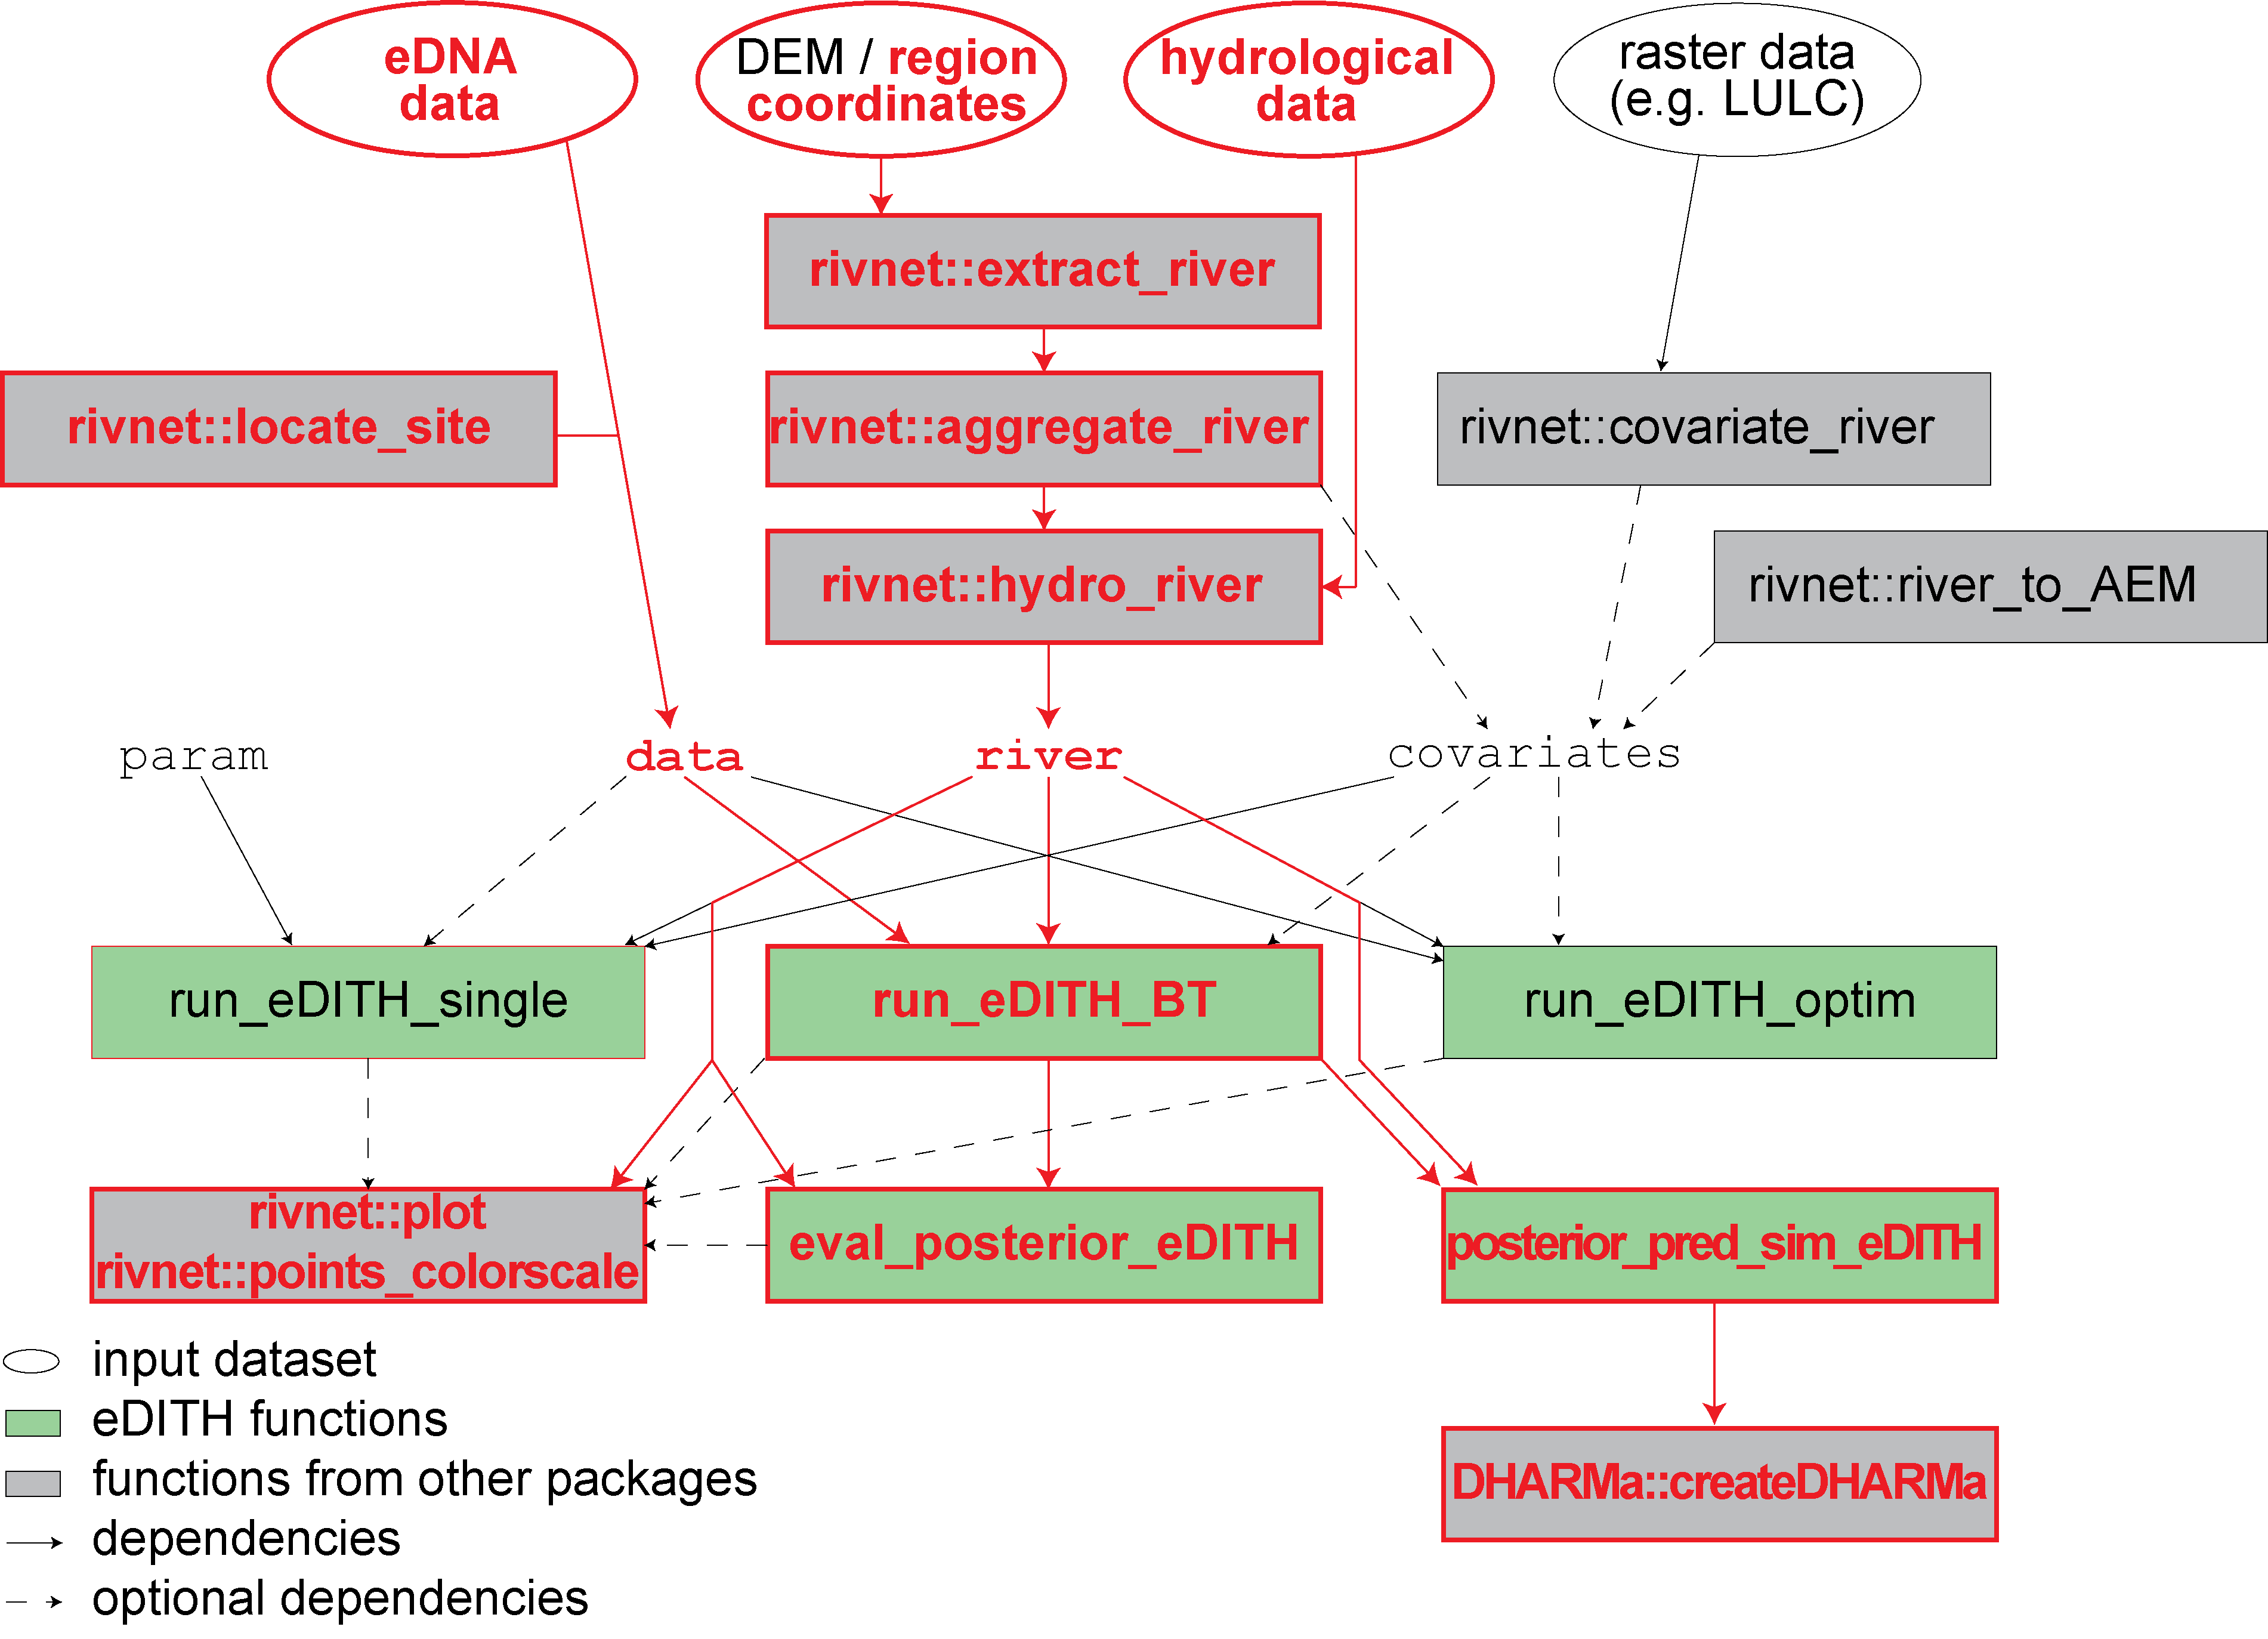
\includegraphics[width=0.9\linewidth]{../data/eDITH_scheme}

\hypertarget{initialization}{%
\section{Initialization}\label{initialization}}

\hypertarget{river-data}{%
\subsection{River data}\label{river-data}}

We stored key information on the river morphology and hydraulics in \texttt{riverData.csv}. Importantly, we do not need to delineate a watershed with external GIS software, nor provide a Digital Elevation Model (DEM) of the regions of interest. Rather, we use \texttt{rivnet} to automatically download open-source DEM data, for which we only need the coordinates of the basins' outlets and of the extent (i.e., lower left and upper right corners) of the DEMs to be downloaded. Internally, DEM data are accessed via a call to the \texttt{elevatr} package, on which \texttt{rivnet} depends.

\begin{Shaded}
\begin{Highlighting}[]
\NormalTok{riverData }\OtherTok{\textless{}{-}} \FunctionTok{read.csv}\NormalTok{(}\AttributeTok{file=}\StringTok{"../data/riverData.csv"}\NormalTok{) }
\NormalTok{riverData}
\CommentTok{\#\textgreater{}      river X.outlet Y.outlet EPSG   X.min   X.max   Y.min   Y.max  z  thrA}
\CommentTok{\#\textgreater{} 1 Sydenham  2970788  8827521 3085 2960831 3039079 8817103 8907142 10 1e+06}
\CommentTok{\#\textgreater{} 2    Koide  1402942  1143218 6684 1402699 1407461 1142792 1155735 10 1e+05}
\CommentTok{\#\textgreater{}   Q.outlet w.outlet}
\CommentTok{\#\textgreater{} 1     34.4       60}
\CommentTok{\#\textgreater{} 2      1.0       15}
\end{Highlighting}
\end{Shaded}

\begin{itemize}
\tightlist
\item
  \texttt{river} provides a tag for the two case studies: \texttt{Sydenham} for (Balasingham et al. 2018) and \texttt{Koide} for (Sakata et al. 2021).
\item
  \texttt{X.outlet}, \texttt{Y.outlet} are the outlet coordinates (longitude and latitude) in the projected coordinate system defined by \texttt{EPSG}. \texttt{EPSG\ =\ 3085} corresponds to the NAD83(HARN) / Texas Centric Albers Equal Area, while \texttt{EPSG\ =\ 6684} corresponds to the JGD2011 / Japan Plane Rectangular CS XVI system. Please refer to \href{https://epsg.org/}{this website} for an overview of EPSG codes. \textbf{It is fundamental that a projected coordinate system (i.e., with coordinate values expressed in meters) is chosen}. In this way, all distances and areas contained in the \texttt{river} object produced by \texttt{rivnet} will be in m and m\^{}2, respectively, which will ensure a correct functioning of \texttt{eDITH} functions.
\item
  \texttt{X.min}, \texttt{X.max}, \texttt{Y.min}, \texttt{Y.max} are the coordinates (in the system specified by \texttt{EPSG}) of the DEM that will be clipped and processed in order to delineate the watershed. \textbf{This region must be at least as wide as (or ideally minimally wider than) the extent of the watershed}, such that the complete watershed can be reconstructed. It is thus advised to provide a large range for these values, especially when the shape of the watershed is not exactly known a priori. Obviously, the drawback of providing too large of a range is that the watershed delineation will be slowed down. However, subsequent processes on the extracted watershed (such as the application of eDITH) are independent of the choice of the initial coordinate range, provided that the watershed has been correctly extracted.
\item
  \texttt{z} is the zoom level at which the DEM will be downloaded. The exact cell size corresponding to a given zoom level depends on the latitude. Details are provided in the documentation of \texttt{elevatr}. \texttt{z\ =\ 10} corresponds to a cell size of about 50 m at the latitudes of the case study catchments. Increasing \texttt{z} by one unit will decrease the cell size by about twofold.
\item
  \texttt{thrA} is the threshold area value (in m\textsuperscript{2}) at which a DEM cell is assumed to be part of the channel network. This value should be small enough such that all headwaters on which eDNA sampling sites were located are contained in the extracted river network; at the same time, too small of a value would generate a river network with too many nodes, which would slow down the execution of eDITH considerably. See also (Carraro and Altermatt 2022). We used a larger \texttt{thrA} value for the Sydenham river because it is a larger watershed.
\item
  \texttt{Q.outlet} and \texttt{w.outlet} are the values of discharge (in m\textsuperscript{3} s\textsuperscript{-1}) and river width (in m) at the outlet, respectively. From these values, \texttt{rivnet}'s \texttt{hydro\_river} can extrapolate hydrological variables needed for application of eDITH to all reaches of the river network. For this application, width values were inferred from aerial images (Google Maps). Mean annual discharge was reported in (Balasingham et al. 2018), while no discharge value was provided in (Sakata et al. 2021). Therefore, we inferred the outlet discharge value by assuming that each km\textsuperscript{2} of drainage area would contribute a discharge of about 0.025 m\textsuperscript{3}s\textsuperscript{-1}, which is reasonable in temperate climates.
\end{itemize}

\hypertarget{initialize-variables}{%
\subsection{Initialize variables}\label{initialize-variables}}

We will use Asymmetric Eigenvector Maps (AEMs) as covariates in the eDITH model. AEMs (Blanchet, Legendre, and Borcard 2008) are mutually orthogonal spatial variables obtained by a spatial filtering technique that considers space in an asymmetric way, and are thus suitable to model species distributions in river networks. The use of AEMs as covariates is convenient because it allows capturing spatial patterns in the data without the need to provide and process raster files to compute geomorphological and/or landcover covariates. See the documentation of \texttt{run\_eDITH\_BT} and \texttt{run\_eDITH\_optim} for examples where such covariates are used.

Specifically, we will only retain the first 10 AEM covariates (sorted in decreasing order by their respective eigenvalue). We will only consider species found in at least 5 sampling sites.

\begin{Shaded}
\begin{Highlighting}[]
\NormalTok{n\_covariates }\OtherTok{\textless{}{-}} \DecValTok{10} \CommentTok{\# number of covariates used in eDITH}
\NormalTok{thr\_species }\OtherTok{\textless{}{-}} \DecValTok{5}   \CommentTok{\# exclude species with \textless{} thr\_species detections from modelling}

\NormalTok{probDet }\OtherTok{\textless{}{-}}\NormalTok{ signifCovariates }\OtherTok{\textless{}{-}} \FunctionTok{vector}\NormalTok{(}\StringTok{"list"}\NormalTok{,}\DecValTok{2}\NormalTok{)}
\NormalTok{gelmanDiag }\OtherTok{\textless{}{-}}\NormalTok{ SST }\OtherTok{\textless{}{-}}\NormalTok{ speciesID }\OtherTok{\textless{}{-}} \FunctionTok{vector}\NormalTok{(}\StringTok{"list"}\NormalTok{,}\DecValTok{2}\NormalTok{)}
\FunctionTok{names}\NormalTok{(probDet) }\OtherTok{\textless{}{-}} \FunctionTok{names}\NormalTok{(signifCovariates) }\OtherTok{\textless{}{-}}\NormalTok{ riverData}\SpecialCharTok{$}\NormalTok{river}
\FunctionTok{names}\NormalTok{(gelmanDiag) }\OtherTok{\textless{}{-}} \FunctionTok{names}\NormalTok{(SST) }\OtherTok{\textless{}{-}} \FunctionTok{names}\NormalTok{(speciesID) }\OtherTok{\textless{}{-}}\NormalTok{ riverData}\SpecialCharTok{$}\NormalTok{river}
\end{Highlighting}
\end{Shaded}

All the following are lists with two objects named \texttt{Sydenham} and \texttt{Koide}.

\begin{itemize}
\tightlist
\item
  \texttt{probDet}: modelled detection probabilities for all species.
\item
  \texttt{signifCovariates}: information on which covariates are significant for which species.
\item
  \texttt{gelmanDiag}: values of the Gelman's diagnostic (provided by \texttt{BayesianTools}).
\item
  \texttt{SST}: species-by-site tables as provided by (Balasingham et al. 2018) and (Sakata et al. 2021)
\item
  \texttt{speciesID}: indices of species with more than \texttt{thr\_species} occurrences, which will actually be modelled.
\end{itemize}

\hypertarget{case-study-1-sydenham-river}{%
\section{Case study 1: Sydenham river}\label{case-study-1-sydenham-river}}

\hypertarget{watershed-delineation}{%
\subsection{Watershed delineation}\label{watershed-delineation}}

We can now use \texttt{rivnet}'s \texttt{extract\_river} to delineate the Sydenham watershed:

\begin{Shaded}
\begin{Highlighting}[]
\NormalTok{ Sydenham }\OtherTok{\textless{}{-}}\NormalTok{ rivnet}\SpecialCharTok{::}\FunctionTok{extract\_river}\NormalTok{(}\AttributeTok{outlet =} \FunctionTok{c}\NormalTok{(riverData}\SpecialCharTok{$}\NormalTok{X.outlet[}\DecValTok{1}\NormalTok{], }
\NormalTok{                                              riverData}\SpecialCharTok{$}\NormalTok{Y.outlet[}\DecValTok{1}\NormalTok{]),}
                                   \AttributeTok{EPSG =}\NormalTok{ riverData}\SpecialCharTok{$}\NormalTok{EPSG[}\DecValTok{1}\NormalTok{],}
                                   \AttributeTok{ext =} \FunctionTok{c}\NormalTok{(riverData}\SpecialCharTok{$}\NormalTok{X.min[}\DecValTok{1}\NormalTok{], }
\NormalTok{                                           riverData}\SpecialCharTok{$}\NormalTok{X.max[}\DecValTok{1}\NormalTok{],}
\NormalTok{                                           riverData}\SpecialCharTok{$}\NormalTok{Y.min[}\DecValTok{1}\NormalTok{], }
\NormalTok{                                           riverData}\SpecialCharTok{$}\NormalTok{Y.max[}\DecValTok{1}\NormalTok{]),}
                                   \AttributeTok{z =}\NormalTok{ riverData}\SpecialCharTok{$}\NormalTok{z[}\DecValTok{1}\NormalTok{],}
                                   \AttributeTok{showPlot =}\NormalTok{ T,          }
                                   \AttributeTok{threshold\_parameter =} \DecValTok{1000}\NormalTok{, }
                                   \AttributeTok{displayUpdates =} \DecValTok{1}\NormalTok{,    }
                                   \AttributeTok{n\_processes =} \DecValTok{8}\NormalTok{)       }
\CommentTok{\#\textgreater{} Remove pits...}
\CommentTok{\#\textgreater{} D8 flow directions...}
\CommentTok{\#\textgreater{} Contributing areas...}
\CommentTok{\#\textgreater{} Stream definition by threshold...}
\CommentTok{\#\textgreater{} Move outlet to stream...}
\CommentTok{\#\textgreater{} Contributing area upstream of outlet...}
\end{Highlighting}
\end{Shaded}

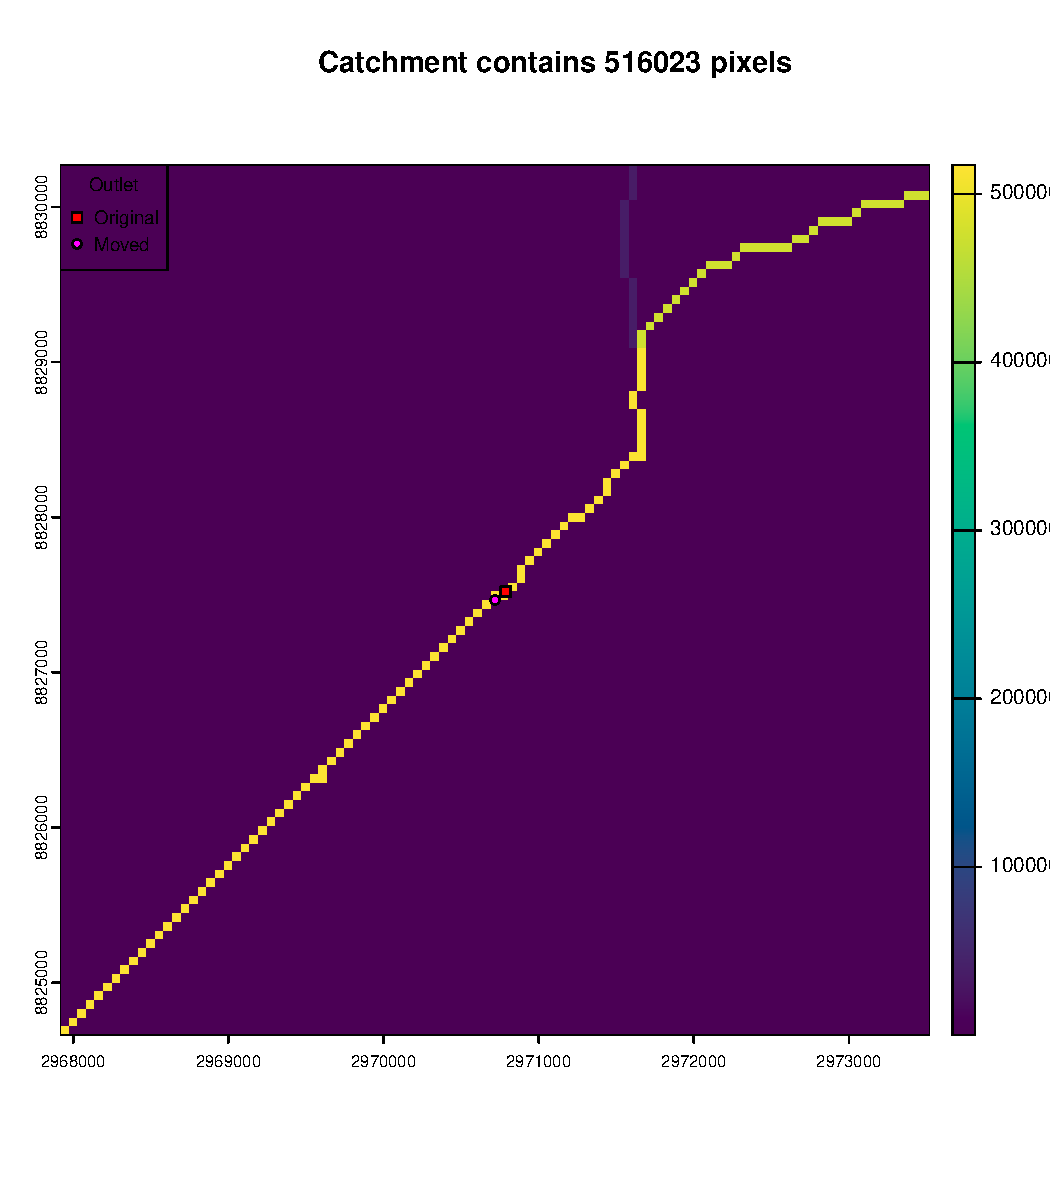
\includegraphics{Illustrating_eDITH_files/figure-latex/unnamed-chunk-5-1.pdf}

\begin{verbatim}
#> Creation of river object...
#> Creation of river object... 100.0%
#> extract_river has finished.
#> Time for DEM download: 7.4 s
#> Time for TauDEM processing: 182.0 s
#> Time for creation of river object: 5.8 s
\end{verbatim}

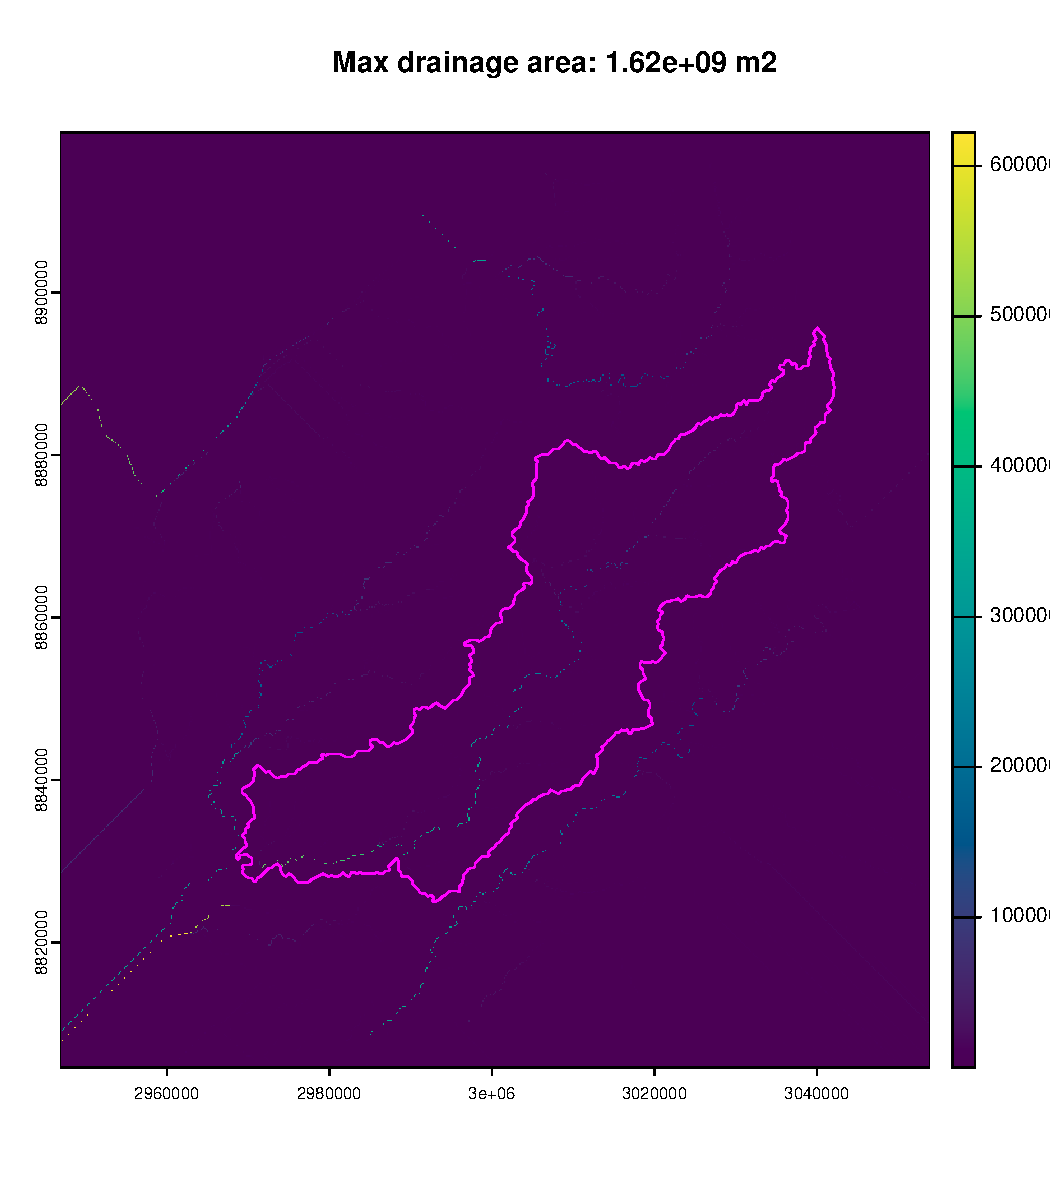
\includegraphics{Illustrating_eDITH_files/figure-latex/unnamed-chunk-5-2.pdf}

\begin{Shaded}
\begin{Highlighting}[]
\CommentTok{\# showPlot = T: display figures}
\CommentTok{\# threshold\_parameter = 1000: minimum cell number to identify channels}
\CommentTok{\#                             only used to snap the outlet to the river network}
\CommentTok{\# displayUpdates = 1: display updates on console}
\CommentTok{\# n\_processes = 8: enable parallel computing with 8 processors}
\end{Highlighting}
\end{Shaded}

Using \texttt{showPlot\ =\ T} produced two figures, which we can use to identify possible issues in the delineation of a watershed. The first one shows a zoom-in in the proximity of the outlet. The coordinates of the original (i.e., provided by the user) and moved outlet (i.e., snapped to the river network) are shown. Values displayed with colors are drainage areas (in number of cells). Blue cells are cells not belonging to the river network, while yellow cells identify the river network. \textbf{If the river appears white, it means that the corresponding cells have a NaN value of drainage area. This signals that something went wrong in the watershed delineation}. Most probably, the range provided in \texttt{ext} was not sufficient to contain the whole catchment. The second figure shows a drainage area map of the whole region (as specified in \texttt{ext}), with the derived watershed contour in magenta.

The so-obtained object of \texttt{river} class can be aggregated into reaches via \texttt{aggregate\_river}:

\begin{Shaded}
\begin{Highlighting}[]
\NormalTok{Sydenham}
\CommentTok{\#\textgreater{} Class         : river }
\CommentTok{\#\textgreater{} Type          : Real river }
\CommentTok{\#\textgreater{} No. FD nodes  : 516023 }
\CommentTok{\#\textgreater{} Dimensions    : 1909 x 2052 }
\CommentTok{\#\textgreater{} Cell size     : 56.09 }
\CommentTok{\#\textgreater{} Has elevation : TRUE }
\CommentTok{\#\textgreater{} Aggregated    : FALSE}
\NormalTok{Sydenham }\OtherTok{\textless{}{-}}\NormalTok{ rivnet}\SpecialCharTok{::}\FunctionTok{aggregate\_river}\NormalTok{(Sydenham, }\AttributeTok{thrA=}\NormalTok{riverData}\SpecialCharTok{$}\NormalTok{thrA[}\DecValTok{1}\NormalTok{],}
                                    \AttributeTok{maxReachLength=}\DecValTok{1000}\NormalTok{,}
                                    \AttributeTok{equalizeLengths=}\ConstantTok{TRUE}\NormalTok{)}
\NormalTok{Sydenham}
\CommentTok{\#\textgreater{} Class         : river }
\CommentTok{\#\textgreater{} Type          : Real river }
\CommentTok{\#\textgreater{} No. FD nodes  : 516023 }
\CommentTok{\#\textgreater{} Dimensions    : 1909 x 2052 }
\CommentTok{\#\textgreater{} Cell size     : 56.09 }
\CommentTok{\#\textgreater{} Has elevation : TRUE }
\CommentTok{\#\textgreater{} Aggregated    : TRUE }
\CommentTok{\#\textgreater{}    Threshold area  : 1000000.00 }
\CommentTok{\#\textgreater{}    Max reach length: 1000.00 }
\CommentTok{\#\textgreater{}    No. RN nodes    : 18375 }
\CommentTok{\#\textgreater{}    No. AG nodes    : 1715 }
\CommentTok{\#\textgreater{}    Has paths       :  FALSE }
\CommentTok{\#\textgreater{}    River geometry  :  FALSE}
\end{Highlighting}
\end{Shaded}

We imposed a maximum reach length of 1000 m, and forced the algorithm to split longer reaches in portions of (approximately) equal length.

\begin{Shaded}
\begin{Highlighting}[]
\NormalTok{Sydenham}\SpecialCharTok{$}\NormalTok{AG}\SpecialCharTok{$}\NormalTok{nNodes}
\CommentTok{\#\textgreater{} [1] 1715}
\end{Highlighting}
\end{Shaded}

The extracted river consists of 1715 nodes at the AG level.

\hypertarget{hydrological-characterization}{%
\subsection{Hydrological characterization}\label{hydrological-characterization}}

Function \texttt{hydro\_river} of \texttt{rivnet} can be used to extrapolate hydrological variables across the river network. We first define a data frame containing the necessary data (see \texttt{hydro\_river}'s documentation for details), and then call \texttt{hydro\_river}:

\begin{Shaded}
\begin{Highlighting}[]
\NormalTok{hd }\OtherTok{\textless{}{-}} \FunctionTok{data.frame}\NormalTok{(}\AttributeTok{data=}\FunctionTok{c}\NormalTok{(riverData}\SpecialCharTok{$}\NormalTok{Q.outlet[}\DecValTok{1}\NormalTok{], riverData}\SpecialCharTok{$}\NormalTok{w.outlet[}\DecValTok{1}\NormalTok{]),}
                 \AttributeTok{type=}\FunctionTok{c}\NormalTok{(}\StringTok{"Q"}\NormalTok{, }\StringTok{"w"}\NormalTok{),}
                 \AttributeTok{node=}\FunctionTok{c}\NormalTok{(}\DecValTok{1}\NormalTok{,}\DecValTok{1}\NormalTok{)}\SpecialCharTok{*}\NormalTok{Sydenham}\SpecialCharTok{$}\NormalTok{AG}\SpecialCharTok{$}\NormalTok{outlet)}
\NormalTok{Sydenham }\OtherTok{\textless{}{-}} \FunctionTok{hydro\_river}\NormalTok{(hd, Sydenham)}
\end{Highlighting}
\end{Shaded}

Extrapolated discharge values across the river network can be displayed via \texttt{plot()}:

\begin{Shaded}
\begin{Highlighting}[]
\FunctionTok{plot}\NormalTok{(Sydenham}\SpecialCharTok{$}\NormalTok{AG}\SpecialCharTok{$}\NormalTok{discharge, Sydenham)}
\FunctionTok{title}\NormalTok{(}\StringTok{\textquotesingle{}Discharge [m\^{}3 s\^{}{-}1]\textquotesingle{}}\NormalTok{)}
\end{Highlighting}
\end{Shaded}

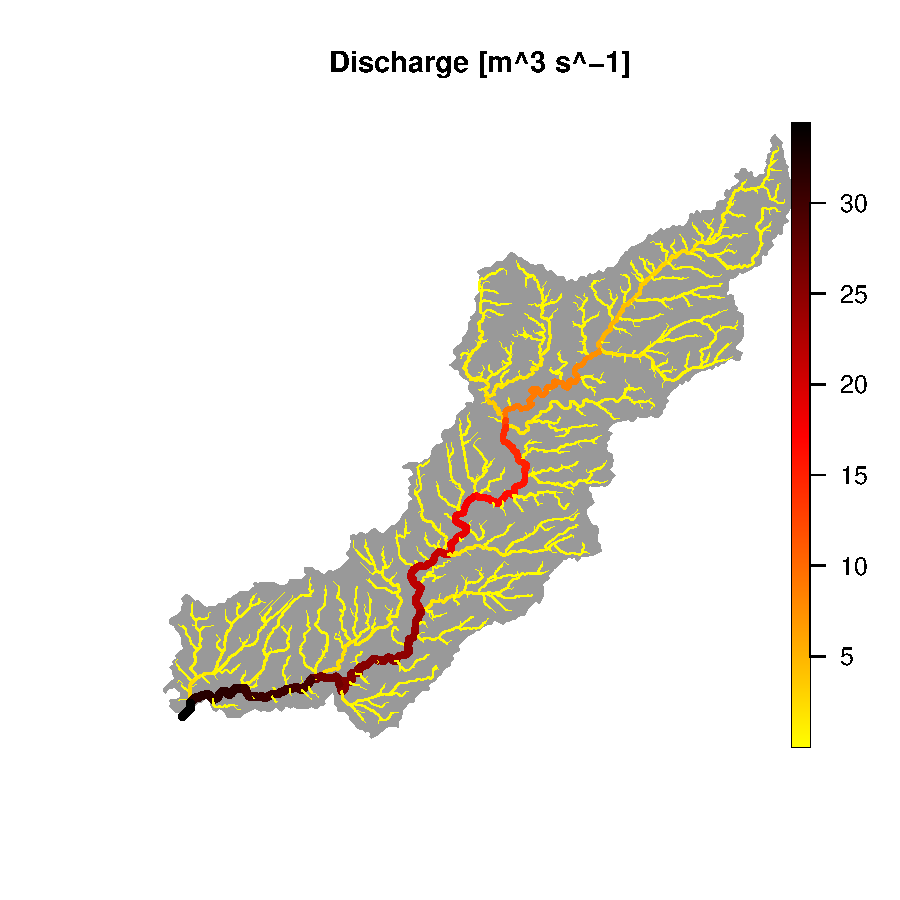
\includegraphics{Illustrating_eDITH_files/figure-latex/unnamed-chunk-9-1.pdf}

\hypertarget{pinpoiting-sampling-sites-to-the-river-reaches}{%
\subsection{Pinpoiting sampling sites to the river reaches}\label{pinpoiting-sampling-sites-to-the-river-reaches}}

Sampling sites' coordinates are contained in \texttt{samplingSitesSydenham.csv}. We can use \texttt{locate\_site} from \texttt{rivnet} to identify the AG nodes (i.e., reaches) associated to the sampling sites.

\begin{Shaded}
\begin{Highlighting}[]
\NormalTok{samplingSitesSydenham }\OtherTok{\textless{}{-}} \FunctionTok{read.csv}\NormalTok{(}\AttributeTok{file=}\StringTok{"../data/samplingSitesSydenham.csv"}\NormalTok{)}

\NormalTok{AGnode }\OtherTok{\textless{}{-}} \FunctionTok{numeric}\NormalTok{(}\FunctionTok{length}\NormalTok{(samplingSitesSydenham}\SpecialCharTok{$}\NormalTok{X))}
\ControlFlowTok{for}\NormalTok{ (j }\ControlFlowTok{in} \DecValTok{1}\SpecialCharTok{:} \FunctionTok{length}\NormalTok{(samplingSitesSydenham}\SpecialCharTok{$}\NormalTok{X))\{}
\NormalTok{  tmp }\OtherTok{\textless{}{-}}\NormalTok{ rivnet}\SpecialCharTok{::}\FunctionTok{locate\_site}\NormalTok{(samplingSitesSydenham}\SpecialCharTok{$}\NormalTok{X[j], }
\NormalTok{                             samplingSitesSydenham}\SpecialCharTok{$}\NormalTok{Y[j], }
\NormalTok{                             Sydenham, }
                             \AttributeTok{showPlot =}\NormalTok{ F)}
\NormalTok{  AGnode[j] }\OtherTok{\textless{}{-}}\NormalTok{ tmp}\SpecialCharTok{$}\NormalTok{AGnode}
\NormalTok{\}}
\end{Highlighting}
\end{Shaded}

In this case, we automatically assigned the closest reach as the crow flies to each sampling site. However, it can happen that, due to discrepancies between the extracted river network and the actual river network, such an automatic assignment would pinpoint a sampling site to a wrong reach. To have a better control over this operation, one can use \texttt{showPlot\ =\ TRUE} in \texttt{locate\_site}. For instance, for the first sampling site:

\begin{Shaded}
\begin{Highlighting}[]
\NormalTok{rivnet}\SpecialCharTok{::}\FunctionTok{locate\_site}\NormalTok{(samplingSitesSydenham}\SpecialCharTok{$}\NormalTok{X[}\DecValTok{1}\NormalTok{], }
\NormalTok{                    samplingSitesSydenham}\SpecialCharTok{$}\NormalTok{Y[}\DecValTok{1}\NormalTok{],}
\NormalTok{                    Sydenham, }
                    \AttributeTok{showPlot =}\NormalTok{ T)}
\FunctionTok{title}\NormalTok{(samplingSitesSydenham}\SpecialCharTok{$}\NormalTok{siteID[}\DecValTok{1}\NormalTok{])}
\end{Highlighting}
\end{Shaded}

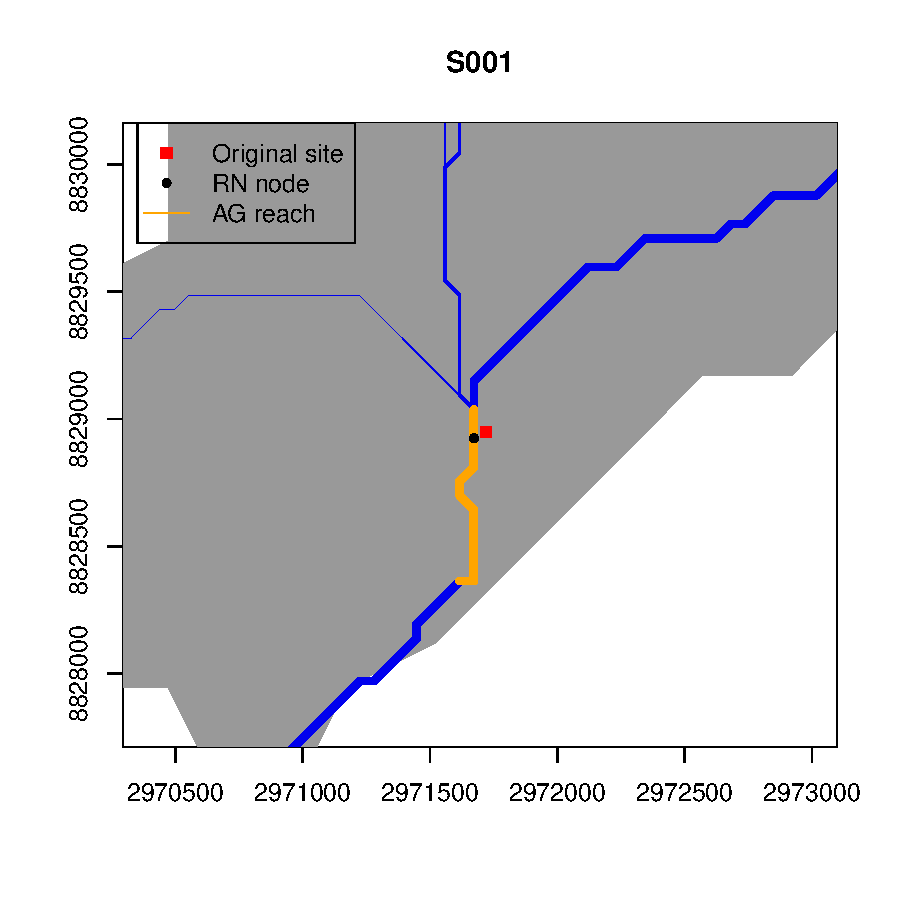
\includegraphics{Illustrating_eDITH_files/figure-latex/unnamed-chunk-11-1.pdf}

In this case, the reach assignation was correct. Conversely, site 10 is wrongly assigned to a tributary, instead of the main stem:

\begin{Shaded}
\begin{Highlighting}[]
\NormalTok{rivnet}\SpecialCharTok{::}\FunctionTok{locate\_site}\NormalTok{(samplingSitesSydenham}\SpecialCharTok{$}\NormalTok{X[}\DecValTok{10}\NormalTok{], }
\NormalTok{                    samplingSitesSydenham}\SpecialCharTok{$}\NormalTok{Y[}\DecValTok{10}\NormalTok{], }
\NormalTok{                    Sydenham, }
                    \AttributeTok{showPlot =}\NormalTok{ T)}
\FunctionTok{title}\NormalTok{(samplingSitesSydenham}\SpecialCharTok{$}\NormalTok{siteID[}\DecValTok{10}\NormalTok{])}
\end{Highlighting}
\end{Shaded}

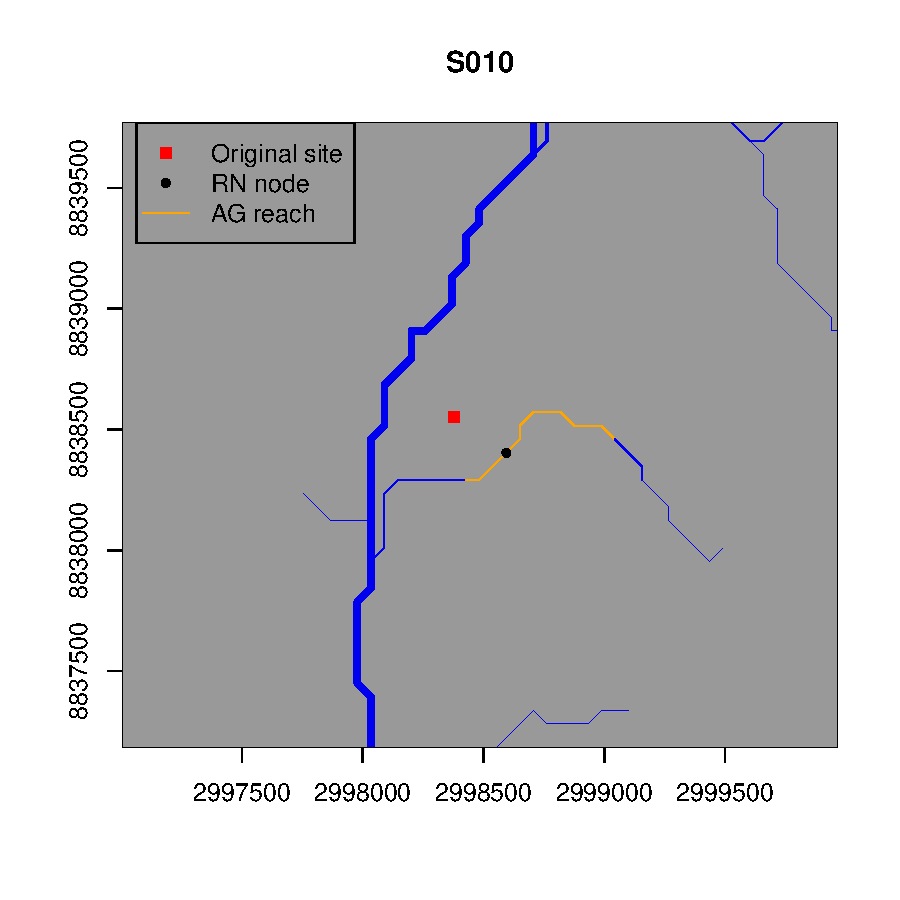
\includegraphics{Illustrating_eDITH_files/figure-latex/unnamed-chunk-12-1.pdf}

Since the topology of the extracted river network cannot be easily changed, the fastest alternative is to tweak the coordinates of the sampling sites so that they are attributed to the correct reach. In this case, we slightly shift site 10 westwards to make it snap to the main stem:

\begin{Shaded}
\begin{Highlighting}[]
\NormalTok{samplingSitesSydenham}\SpecialCharTok{$}\NormalTok{X[}\DecValTok{10}\NormalTok{] }\OtherTok{\textless{}{-}}\NormalTok{ samplingSitesSydenham}\SpecialCharTok{$}\NormalTok{X[}\DecValTok{10}\NormalTok{] }\SpecialCharTok{{-}} \DecValTok{200}
\NormalTok{tmp }\OtherTok{\textless{}{-}}\NormalTok{ rivnet}\SpecialCharTok{::}\FunctionTok{locate\_site}\NormalTok{(samplingSitesSydenham}\SpecialCharTok{$}\NormalTok{X[}\DecValTok{10}\NormalTok{], }
\NormalTok{                           samplingSitesSydenham}\SpecialCharTok{$}\NormalTok{Y[}\DecValTok{10}\NormalTok{], }
\NormalTok{                           Sydenham, }
                           \AttributeTok{showPlot =}\NormalTok{ T)}
\FunctionTok{title}\NormalTok{(samplingSitesSydenham}\SpecialCharTok{$}\NormalTok{siteID[}\DecValTok{10}\NormalTok{])}
\end{Highlighting}
\end{Shaded}

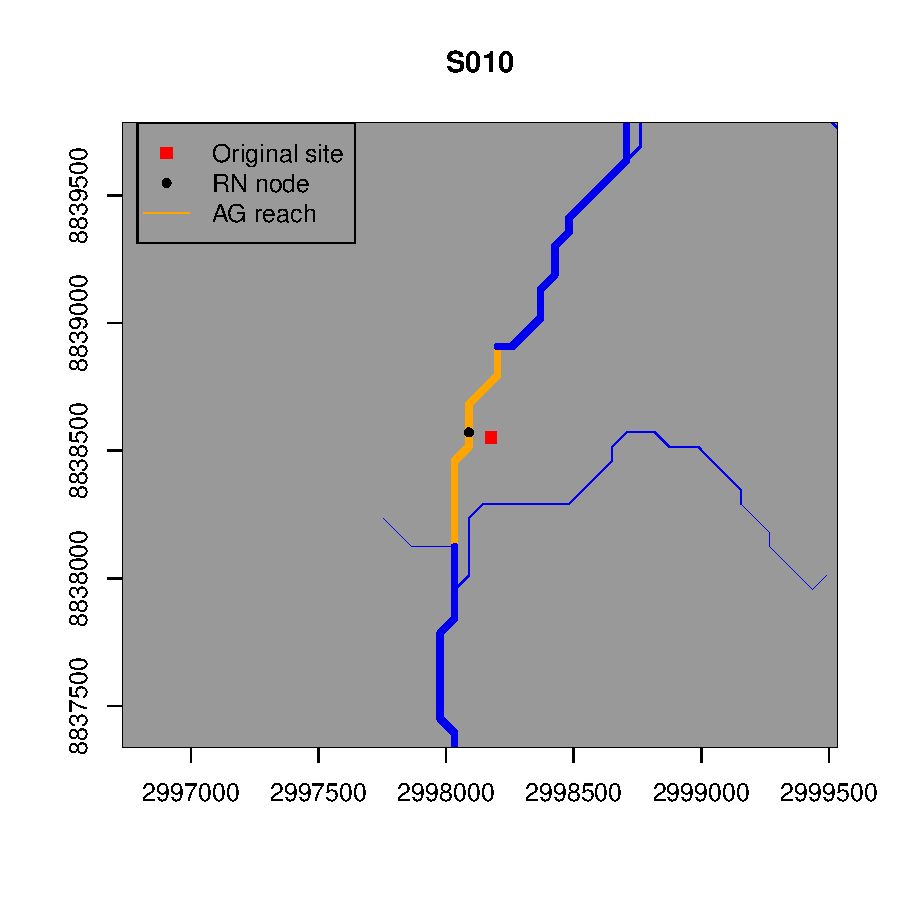
\includegraphics{Illustrating_eDITH_files/figure-latex/unnamed-chunk-13-1.pdf}

\begin{Shaded}
\begin{Highlighting}[]
\NormalTok{AGnode[}\DecValTok{10}\NormalTok{] }\OtherTok{\textless{}{-}}\NormalTok{ tmp}\SpecialCharTok{$}\NormalTok{AGnode}
\end{Highlighting}
\end{Shaded}

All other sampling sites were snapped to the correct reach. We can now store these data:

\begin{Shaded}
\begin{Highlighting}[]
\NormalTok{samplingSitesSydenham[[}\StringTok{"AGnode"}\NormalTok{]] }\OtherTok{\textless{}{-}}\NormalTok{ AGnode}
\end{Highlighting}
\end{Shaded}

\hypertarget{apply-the-edith-model}{%
\subsection{Apply the eDITH model}\label{apply-the-edith-model}}

\hypertarget{initialization-1}{%
\subsubsection{Initialization}\label{initialization-1}}

Read counts are contained in \texttt{siteSpeciesTableSydenham.csv}. The following are the species with at least \texttt{thr\_species} detections:

\begin{Shaded}
\begin{Highlighting}[]
\CommentTok{\# read species{-}by{-}site table}
\NormalTok{SST}\SpecialCharTok{$}\NormalTok{Sydenham }\OtherTok{\textless{}{-}} \FunctionTok{read.csv}\NormalTok{(}\StringTok{"../data/siteSpeciesTableSydenham.csv"}\NormalTok{)}
\NormalTok{SST}\SpecialCharTok{$}\NormalTok{Sydenham[}\FunctionTok{is.na}\NormalTok{(SST}\SpecialCharTok{$}\NormalTok{Sydenham)] }\OtherTok{\textless{}{-}} \DecValTok{0} \CommentTok{\# change NAs to zeros}
\CommentTok{\# choose species with at least thr\_species presences}
\NormalTok{speciesID}\SpecialCharTok{$}\NormalTok{Sydenham }\OtherTok{\textless{}{-}} \FunctionTok{which}\NormalTok{(}\FunctionTok{rowSums}\NormalTok{(SST}\SpecialCharTok{$}\NormalTok{Sydenham[,}\SpecialCharTok{{-}}\DecValTok{1}\NormalTok{]}\SpecialCharTok{!=}\DecValTok{0}\NormalTok{) }\SpecialCharTok{\textgreater{}=}\NormalTok{ thr\_species) }
\NormalTok{SST}\SpecialCharTok{$}\NormalTok{Sydenham[speciesID}\SpecialCharTok{$}\NormalTok{Sydenham,}\DecValTok{1}\NormalTok{]}
\CommentTok{\#\textgreater{}  [1] "Esox lucius"              "Cottus cognatus"         }
\CommentTok{\#\textgreater{}  [3] "Cottus bairdii"           "Percina maculata"        }
\CommentTok{\#\textgreater{}  [5] "Noturus stigmosus"        "Noturus flavus"          }
\CommentTok{\#\textgreater{}  [7] "Nocomis biguttatus"       "Etheostoma blennioides"  }
\CommentTok{\#\textgreater{}  [9] "Semotilus atromaculatus"  "Oncorhynchus tshawytscha"}
\CommentTok{\#\textgreater{} [11] "Pimephales notatus"       "Ambloplites rupestris"   }
\CommentTok{\#\textgreater{} [13] "Culaea inconstans"        "Etheostoma nigrum"       }
\CommentTok{\#\textgreater{} [15] "Ictalurus punctatus"      "Hypentelium nigricans"   }
\CommentTok{\#\textgreater{} [17] "Luxilus cornutus"         "Catostomus commersonii"  }
\CommentTok{\#\textgreater{} [19] "Moxostoma anisurum"       "Moxostoma erythrurum"    }
\CommentTok{\#\textgreater{} [21] "Cyprinus carpio"          "Neogobius melanostomus"}
\end{Highlighting}
\end{Shaded}

We now initialize the export variables for the Sydenham river.

\begin{Shaded}
\begin{Highlighting}[]
\CommentTok{\# initialize variables for export}
\NormalTok{probDet}\SpecialCharTok{$}\NormalTok{Sydenham }\OtherTok{\textless{}{-}} \FunctionTok{data.frame}\NormalTok{(}\FunctionTok{matrix}\NormalTok{(}\DecValTok{0}\NormalTok{, Sydenham}\SpecialCharTok{$}\NormalTok{AG}\SpecialCharTok{$}\NormalTok{nNodes, }
                                      \FunctionTok{length}\NormalTok{(speciesID}\SpecialCharTok{$}\NormalTok{Sydenham)))}
\FunctionTok{names}\NormalTok{(probDet}\SpecialCharTok{$}\NormalTok{Sydenham) }\OtherTok{\textless{}{-}}\NormalTok{ SST}\SpecialCharTok{$}\NormalTok{Sydenham[speciesID[[}\DecValTok{1}\NormalTok{]],}\DecValTok{1}\NormalTok{]}

\NormalTok{signifCovariates}\SpecialCharTok{$}\NormalTok{Sydenham }\OtherTok{\textless{}{-}} \FunctionTok{data.frame}\NormalTok{(}\FunctionTok{matrix}\NormalTok{(}\DecValTok{0}\NormalTok{,n\_covariates, }
                                               \FunctionTok{length}\NormalTok{(speciesID}\SpecialCharTok{$}\NormalTok{Sydenham)))}
\FunctionTok{names}\NormalTok{(signifCovariates}\SpecialCharTok{$}\NormalTok{Sydenham) }\OtherTok{\textless{}{-}}\NormalTok{ SST}\SpecialCharTok{$}\NormalTok{Sydenham[speciesID}\SpecialCharTok{$}\NormalTok{Sydenham,}\DecValTok{1}\NormalTok{]}

\FunctionTok{row.names}\NormalTok{(signifCovariates}\SpecialCharTok{$}\NormalTok{Sydenham) }\OtherTok{\textless{}{-}} \FunctionTok{paste0}\NormalTok{(}\StringTok{"beta\_AEM"}\NormalTok{,}\DecValTok{1}\SpecialCharTok{:}\NormalTok{n\_covariates)}
\NormalTok{gelmanDiag}\SpecialCharTok{$}\NormalTok{Sydenham }\OtherTok{\textless{}{-}} \FunctionTok{data.frame}\NormalTok{(}\FunctionTok{matrix}\NormalTok{(}\DecValTok{0}\NormalTok{,n\_covariates}\SpecialCharTok{+}\DecValTok{3}\NormalTok{,}
                                         \FunctionTok{length}\NormalTok{(speciesID}\SpecialCharTok{$}\NormalTok{Sydenham)))}

\FunctionTok{names}\NormalTok{(gelmanDiag}\SpecialCharTok{$}\NormalTok{Sydenham) }\OtherTok{\textless{}{-}}\NormalTok{ SST}\SpecialCharTok{$}\NormalTok{Sydenham[speciesID}\SpecialCharTok{$}\NormalTok{Sydenham,}\DecValTok{1}\NormalTok{]}
\FunctionTok{row.names}\NormalTok{(gelmanDiag}\SpecialCharTok{$}\NormalTok{Sydenham) }\OtherTok{\textless{}{-}} \FunctionTok{c}\NormalTok{(}\StringTok{"tau"}\NormalTok{,}\StringTok{"log\_p0"}\NormalTok{,}
                                    \FunctionTok{paste0}\NormalTok{(}\StringTok{"beta\_AEM"}\NormalTok{,}\DecValTok{1}\SpecialCharTok{:}\NormalTok{n\_covariates),}\StringTok{"omega"}\NormalTok{)}
\end{Highlighting}
\end{Shaded}

In the last command, we manually included the names of the model parameters. The first two parameters \texttt{tau}and \texttt{log\_p0} refer to the decay time and the logarithm in base 10 of the baseline production rate, respectively. Given that we will use the first 10 AEMs as covariates, parameters for the covariate effect sizes are termed \texttt{beta\_AEM1}, \ldots, \texttt{beta\_AEM10}. Finally, \texttt{omega} is the overdispersion parameter used to control the variance of the negative binomial distribution that we will use to model errors between observed and modelled read counts.

\hypertarget{run-edith-for-a-single-species}{%
\subsubsection{Run eDITH for a single species}\label{run-edith-for-a-single-species}}

We are now ready to run the eDITH model. As an example, let's select the 3rd species:

\begin{Shaded}
\begin{Highlighting}[]
\NormalTok{iS }\OtherTok{\textless{}{-}} \DecValTok{3}
\NormalTok{indSp }\OtherTok{\textless{}{-}}\NormalTok{ speciesID}\SpecialCharTok{$}\NormalTok{Sydenham[iS]}
\NormalTok{nam }\OtherTok{\textless{}{-}}\NormalTok{ SST}\SpecialCharTok{$}\NormalTok{Sydenham[indSp,}\DecValTok{1}\NormalTok{]}
\NormalTok{nam}
\CommentTok{\#\textgreater{} [1] "Cottus bairdii"}
\end{Highlighting}
\end{Shaded}

We create the \texttt{data} data frame containing IDs of the sampling sites and the respective eDNA values:

\begin{Shaded}
\begin{Highlighting}[]
\NormalTok{values }\OtherTok{\textless{}{-}} \FunctionTok{as.numeric}\NormalTok{(SST}\SpecialCharTok{$}\NormalTok{Sydenham[indSp,}\SpecialCharTok{{-}}\DecValTok{1}\NormalTok{]) }
\CommentTok{\# final "{-}1" to get rid of the species name }
\CommentTok{\# as.numeric() to only deal with numeric values }
\NormalTok{data }\OtherTok{\textless{}{-}} \FunctionTok{data.frame}\NormalTok{(}\AttributeTok{ID=}\NormalTok{samplingSitesSydenham}\SpecialCharTok{$}\NormalTok{AGnode, }\AttributeTok{values=}\NormalTok{values) }
\end{Highlighting}
\end{Shaded}

We can now call \texttt{run\_eDITH\_BT}. We do not specify any \texttt{covariates}, since we are going to use the first 10 AEMs for this purpose. Specifically, we will use exponential weights to define the AEMs (see documentation of \texttt{OCN\_to\_AEM} of package \texttt{OCNet} for details). We define a negative binomial error distribution (\texttt{ll.type\ =\ "nbinom"}). We use default settings with respect to prior distributions and options for the MCMC sampler. Depending on the processor used, this step should take about 1 hour to complete.

\begin{Shaded}
\begin{Highlighting}[]
\NormalTok{out }\OtherTok{\textless{}{-}} \FunctionTok{run\_eDITH\_BT}\NormalTok{(data, Sydenham, }\AttributeTok{ll.type=}\StringTok{"nbinom"}\NormalTok{,}
                    \AttributeTok{n.AEM=}\NormalTok{n\_covariates, }\AttributeTok{par.AEM=}\FunctionTok{list}\NormalTok{(}\AttributeTok{weight=}\StringTok{"exponential"}\NormalTok{),}
                    \AttributeTok{verbose=}\NormalTok{T)}
\end{Highlighting}
\end{Shaded}

\hypertarget{analyze-edith-output}{%
\paragraph{Analyze eDITH output}\label{analyze-edith-output}}

After \texttt{run\_eDITH\_BT} has completed, we now use \texttt{eval\_posterior\_eDITH} to evaluate relevant quantiles from the posterior distribution. Specifically, we are interested in the posterior median and in the 2.5th-97.5th percentiles:

\begin{Shaded}
\begin{Highlighting}[]
\NormalTok{out }\OtherTok{\textless{}{-}} \FunctionTok{eval\_posterior\_eDITH}\NormalTok{(out, Sydenham, }\AttributeTok{quant=}\FunctionTok{c}\NormalTok{(}\FloatTok{0.025}\NormalTok{, }\FloatTok{0.5}\NormalTok{, }\FloatTok{0.975}\NormalTok{))}
\end{Highlighting}
\end{Shaded}

Let's now run posterior predictive simulations via \texttt{posterior\_pred\_sim\_eDITH}:

\begin{Shaded}
\begin{Highlighting}[]
\NormalTok{pps }\OtherTok{\textless{}{-}} \FunctionTok{posterior\_pred\_sim\_eDITH}\NormalTok{(out, Sydenham)}
\end{Highlighting}
\end{Shaded}

We can display the posterior median detection probability with \texttt{plot}. This internally calls \texttt{draw\_thematic\_OCN} from \texttt{OCNet}, hence see this function's documentation for a more complete control of its functioning. For instance, we can use \texttt{args\_imagePlot} to pass the colorbar's label.

On top of the river map, we can draw the observed read counts in order to perform a visual check of the soundness of the model fitting. We can do so via \texttt{rivnet}'s \texttt{points\_colorscale}. We can use option \texttt{force.range\ =\ FALSE} to show non-detections (i.e., \texttt{-Inf} values, when the logarithm of observed read numbers is taken) with a transparent background:

\begin{Shaded}
\begin{Highlighting}[]
\FunctionTok{plot}\NormalTok{(out}\SpecialCharTok{$}\NormalTok{probDetection\_quantile[}\DecValTok{2}\NormalTok{,], Sydenham,}
     \AttributeTok{args\_imagePlot=}\FunctionTok{list}\NormalTok{(}\AttributeTok{legend.lab=}\StringTok{"Posterior median detection probability"}\NormalTok{))}
\FunctionTok{title}\NormalTok{(nam)}
\NormalTok{rivnet}\SpecialCharTok{::}\FunctionTok{points\_colorscale}\NormalTok{(samplingSitesSydenham}\SpecialCharTok{$}\NormalTok{X, samplingSitesSydenham}\SpecialCharTok{$}\NormalTok{Y, }
                          \FunctionTok{log10}\NormalTok{(out}\SpecialCharTok{$}\NormalTok{data}\SpecialCharTok{$}\NormalTok{values),}
                          \AttributeTok{force.range =} \ConstantTok{FALSE}\NormalTok{, }
                          \AttributeTok{bg.palette=}\FunctionTok{hcl.colors}\NormalTok{(}\DecValTok{1000}\NormalTok{, }\StringTok{"Blues 3"}\NormalTok{, }\AttributeTok{rev=}\NormalTok{T),}
                          \AttributeTok{horizontal=}\NormalTok{T, }
                          \AttributeTok{legend.lab =} \StringTok{"Observed read counts (log 10)"}\NormalTok{)}
\end{Highlighting}
\end{Shaded}

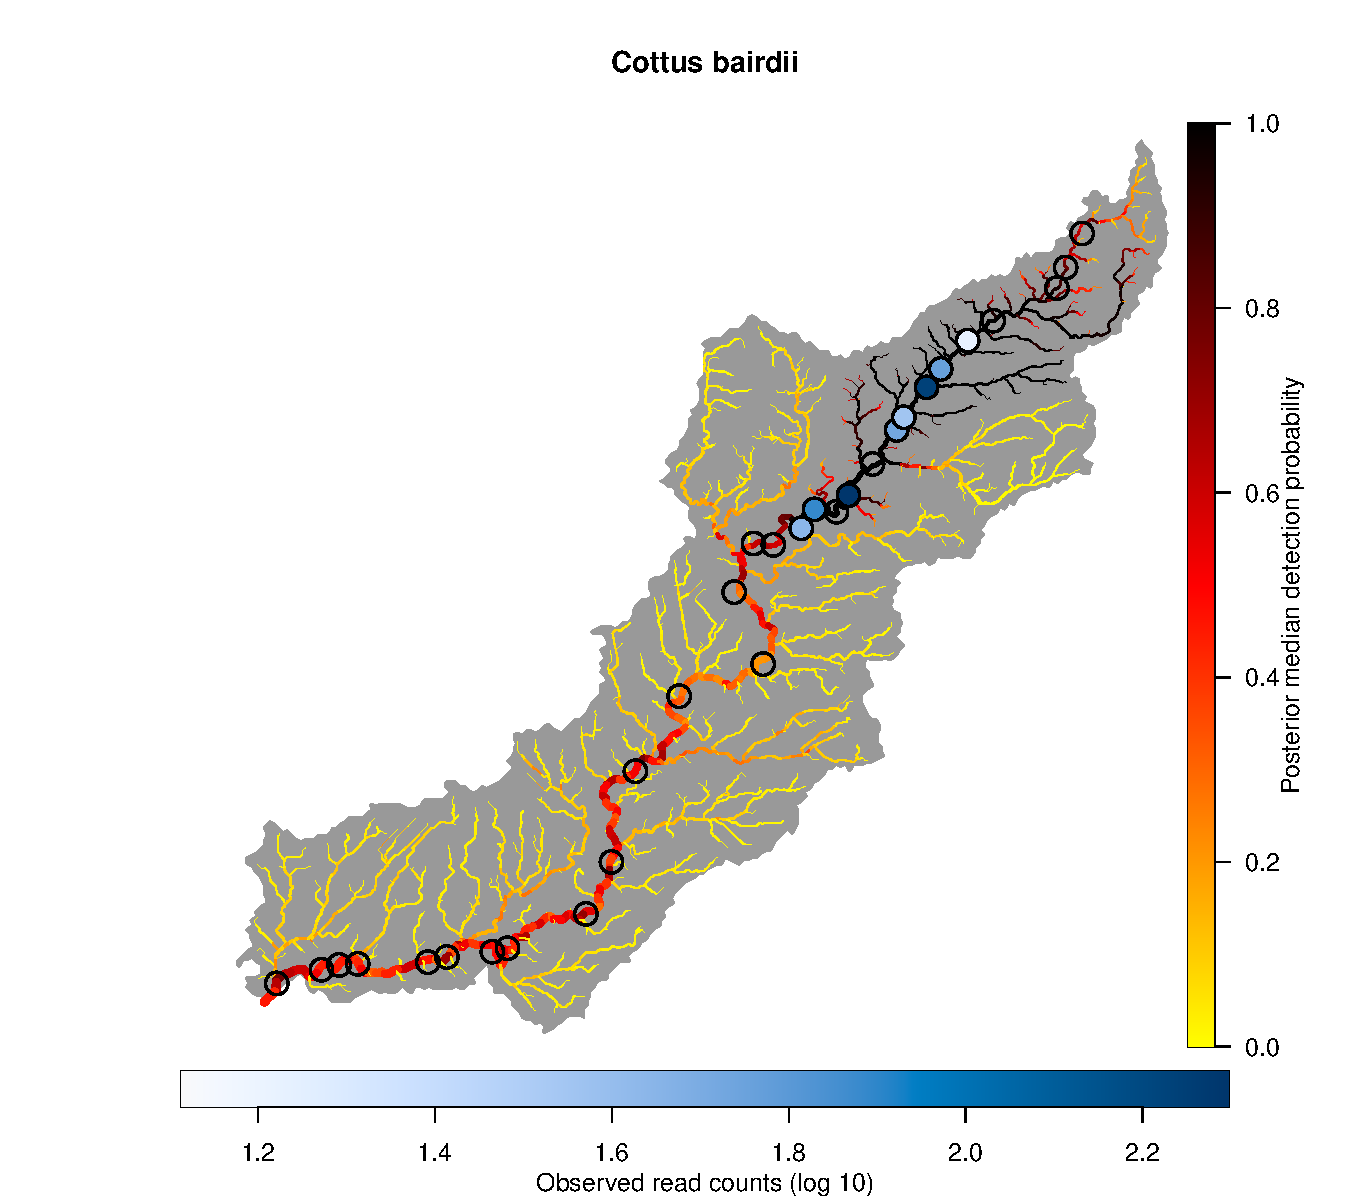
\includegraphics{Illustrating_eDITH_files/figure-latex/unnamed-chunk-23-1.pdf}

Finally, we can use the posterior predictive simulations \texttt{pps} as input in function \texttt{createDHARMa} from \texttt{DHARMa} to explore the goodness of fit of our model. Please refer to the \texttt{DHARMa} documentation for an interpretation of the diagnostics plot.

\begin{Shaded}
\begin{Highlighting}[]
\NormalTok{out.sim }\OtherTok{\textless{}{-}}\NormalTok{ DHARMa}\SpecialCharTok{::}\FunctionTok{createDHARMa}\NormalTok{(pps, out}\SpecialCharTok{$}\NormalTok{data}\SpecialCharTok{$}\NormalTok{values)}
\CommentTok{\#\textgreater{} No fitted predicted response provided, using the mean of the simulations}
\FunctionTok{plot}\NormalTok{(out.sim)}
\end{Highlighting}
\end{Shaded}

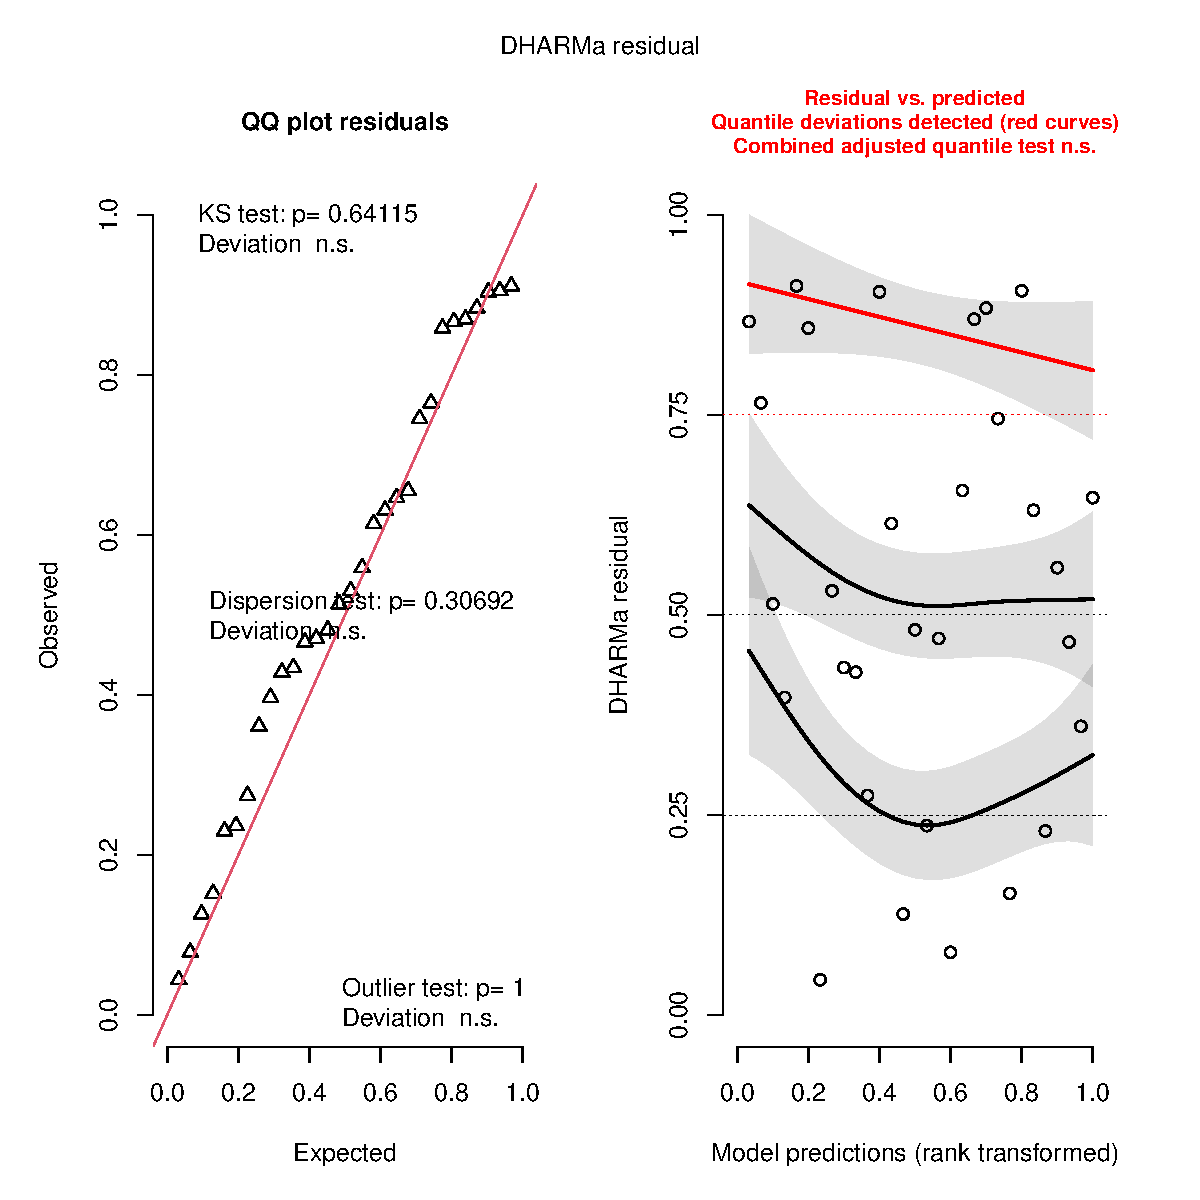
\includegraphics{Illustrating_eDITH_files/figure-latex/unnamed-chunk-24-1.pdf}

\hypertarget{run-edith-for-all-species}{%
\subsubsection{Run eDITH for all species}\label{run-edith-for-all-species}}

The following code loops through all species found (i.e., those with at least \texttt{thr\_species} detections) and runs the eDITH model for each of them. For each species, we export the posterior median detection probability (in \texttt{probDet}), Gelman diagnostics values (\texttt{gelmanDiag}) and information on significant covariates (\texttt{signifCovariates}).

\begin{itemize}
\tightlist
\item
  Gelman diagnostics are calculated within \texttt{BayesianTools}, and provide a metric to assess whether the Markov chains have converged (see the documentation of \texttt{BayesianTools}' \texttt{gelmanDiagnostics} for more details).
\item
  Significant covariates are those for which the equal-tailed 95\% of the corresponding posterior effect size does not overlap 0. If for a given species a certain covariate is significantly positive (i.e., the equal-tailed 95\% of the posterior distribution of the corresponding effect size is positive), the corresponding entry of \texttt{signifCovariates} will contain a \texttt{1}. Negatively significant covariates are marked with \texttt{-1}. Non-significant covariates are marked with \texttt{0}.
\end{itemize}

\begin{Shaded}
\begin{Highlighting}[]
\ControlFlowTok{for}\NormalTok{ (iS }\ControlFlowTok{in} \DecValTok{1}\SpecialCharTok{:}\FunctionTok{length}\NormalTok{(speciesID}\SpecialCharTok{$}\NormalTok{Sydenham))\{ }\CommentTok{\# loop over species}
\NormalTok{  indSp }\OtherTok{\textless{}{-}}\NormalTok{ speciesID}\SpecialCharTok{$}\NormalTok{Sydenham[iS]}
\NormalTok{  nam }\OtherTok{\textless{}{-}}\NormalTok{ SST}\SpecialCharTok{$}\NormalTok{Sydenham[indSp,}\DecValTok{1}\NormalTok{]}
\NormalTok{  fnam }\OtherTok{\textless{}{-}} \FunctionTok{paste0}\NormalTok{(}\StringTok{\textquotesingle{}../resultsSydenham/\textquotesingle{}}\NormalTok{,nam,}\StringTok{\textquotesingle{}.rda\textquotesingle{}}\NormalTok{)}
  
  \ControlFlowTok{if}\NormalTok{(}\SpecialCharTok{!}\FunctionTok{file.exists}\NormalTok{(fnam))\{ }\CommentTok{\# if eDITH results were already generated, skip}
\NormalTok{  values }\OtherTok{\textless{}{-}} \FunctionTok{as.numeric}\NormalTok{(SST}\SpecialCharTok{$}\NormalTok{Sydenham[indSp,}\SpecialCharTok{{-}}\DecValTok{1}\NormalTok{])}
\NormalTok{  data }\OtherTok{\textless{}{-}} \FunctionTok{data.frame}\NormalTok{(}\AttributeTok{ID=}\NormalTok{samplingSitesSydenham}\SpecialCharTok{$}\NormalTok{AGnode, }\AttributeTok{values=}\NormalTok{values) }
  \CommentTok{\# for the species at hand}
  \CommentTok{\# run eDITH model via BayesianTools}
\NormalTok{  out }\OtherTok{\textless{}{-}} \FunctionTok{run\_eDITH\_BT}\NormalTok{(data, Sydenham, }\AttributeTok{ll.type=}\StringTok{"nbinom"}\NormalTok{,}
                      \AttributeTok{n.AEM=}\NormalTok{n\_covariates, }\AttributeTok{par.AEM=}\FunctionTok{list}\NormalTok{(}\AttributeTok{weight=}\StringTok{"exponential"}\NormalTok{),}
                      \AttributeTok{verbose=}\NormalTok{T)}
  \CommentTok{\# evaluate quantiles from posterior distribution}
\NormalTok{  out }\OtherTok{\textless{}{-}} \FunctionTok{eval\_posterior\_eDITH}\NormalTok{(out, Sydenham, }\AttributeTok{quant=}\FunctionTok{c}\NormalTok{(}\FloatTok{0.025}\NormalTok{,}\FloatTok{0.5}\NormalTok{, }\FloatTok{0.975}\NormalTok{))}
  \CommentTok{\# run posterior predictive simulations}
\NormalTok{  pps }\OtherTok{\textless{}{-}} \FunctionTok{posterior\_pred\_sim\_eDITH}\NormalTok{(out, Sydenham)}
  
\NormalTok{  \} }\ControlFlowTok{else}\NormalTok{ \{}\FunctionTok{load}\NormalTok{(fnam)\} }\CommentTok{\# if results already generated, load them}
  
  \CommentTok{\# store posterior median detection probability, }
  \CommentTok{\#   Gelman diagnostics and significance of covariates}
\NormalTok{  probDet}\SpecialCharTok{$}\NormalTok{Sydenham[,iS] }\OtherTok{\textless{}{-}}\NormalTok{ out}\SpecialCharTok{$}\NormalTok{probDetection\_quantile[}\DecValTok{2}\NormalTok{,]}
\NormalTok{  gelmanDiag}\SpecialCharTok{$}\NormalTok{Sydenham[,iS] }\OtherTok{\textless{}{-}}\NormalTok{ out}\SpecialCharTok{$}\NormalTok{gD}\SpecialCharTok{$}\NormalTok{psrf[,}\DecValTok{1}\NormalTok{]}
  \ControlFlowTok{for}\NormalTok{ (j }\ControlFlowTok{in} \DecValTok{1}\SpecialCharTok{:}\FunctionTok{length}\NormalTok{(out}\SpecialCharTok{$}\NormalTok{covariates))\{}
    \ControlFlowTok{if}\NormalTok{ (out}\SpecialCharTok{$}\NormalTok{cI[}\DecValTok{1}\NormalTok{,j}\SpecialCharTok{+}\DecValTok{2}\NormalTok{]}\SpecialCharTok{\textgreater{}}\DecValTok{0}\NormalTok{) signifCovariates}\SpecialCharTok{$}\NormalTok{Sydenham[j,iS] }\OtherTok{\textless{}{-}} \DecValTok{1}
    \ControlFlowTok{if}\NormalTok{ (out}\SpecialCharTok{$}\NormalTok{cI[}\DecValTok{2}\NormalTok{,j}\SpecialCharTok{+}\DecValTok{2}\NormalTok{]}\SpecialCharTok{\textless{}}\DecValTok{0}\NormalTok{) signifCovariates}\SpecialCharTok{$}\NormalTok{Sydenham[j,iS] }\OtherTok{\textless{}{-}} \SpecialCharTok{{-}}\DecValTok{1}
\NormalTok{  \}}
\NormalTok{\}}
\end{Highlighting}
\end{Shaded}

\hypertarget{case-study-2-koide-river}{%
\section{Case study 2: Koide river}\label{case-study-2-koide-river}}

In a similar fashion, we can apply the eDITH model to the dataset of (Sakata et al. 2021).

\hypertarget{watershed-delineation-and-hydrological-characterization}{%
\subsection{Watershed delineation and hydrological characterization}\label{watershed-delineation-and-hydrological-characterization}}

\begin{Shaded}
\begin{Highlighting}[]
\NormalTok{Koide }\OtherTok{\textless{}{-}}\NormalTok{ rivnet}\SpecialCharTok{::}\FunctionTok{extract\_river}\NormalTok{(}\AttributeTok{outlet =} \FunctionTok{c}\NormalTok{(riverData}\SpecialCharTok{$}\NormalTok{X.outlet[}\DecValTok{2}\NormalTok{], }
\NormalTok{                                          riverData}\SpecialCharTok{$}\NormalTok{Y.outlet[}\DecValTok{2}\NormalTok{]),}
                               \AttributeTok{EPSG =}\NormalTok{ riverData}\SpecialCharTok{$}\NormalTok{EPSG[}\DecValTok{2}\NormalTok{],}
                               \AttributeTok{ext =} \FunctionTok{c}\NormalTok{(riverData}\SpecialCharTok{$}\NormalTok{X.min[}\DecValTok{2}\NormalTok{], }
\NormalTok{                                       riverData}\SpecialCharTok{$}\NormalTok{X.max[}\DecValTok{2}\NormalTok{],}
\NormalTok{                                       riverData}\SpecialCharTok{$}\NormalTok{Y.min[}\DecValTok{2}\NormalTok{], }
\NormalTok{                                       riverData}\SpecialCharTok{$}\NormalTok{Y.max[}\DecValTok{2}\NormalTok{]),}
                               \AttributeTok{z =}\NormalTok{ riverData}\SpecialCharTok{$}\NormalTok{z[}\DecValTok{2}\NormalTok{],}
                               \AttributeTok{showPlot =}\NormalTok{ T,}
                               \AttributeTok{threshold\_parameter =} \DecValTok{1000}\NormalTok{,}
                               \AttributeTok{displayUpdates =} \DecValTok{1}\NormalTok{,}
                               \AttributeTok{n\_processes =} \DecValTok{8}\NormalTok{)}
\CommentTok{\#\textgreater{} Remove pits...}
\CommentTok{\#\textgreater{} D8 flow directions...}
\CommentTok{\#\textgreater{} Contributing areas...}
\CommentTok{\#\textgreater{} Stream definition by threshold...}
\CommentTok{\#\textgreater{} Move outlet to stream...}
\CommentTok{\#\textgreater{} Contributing area upstream of outlet...}
\end{Highlighting}
\end{Shaded}

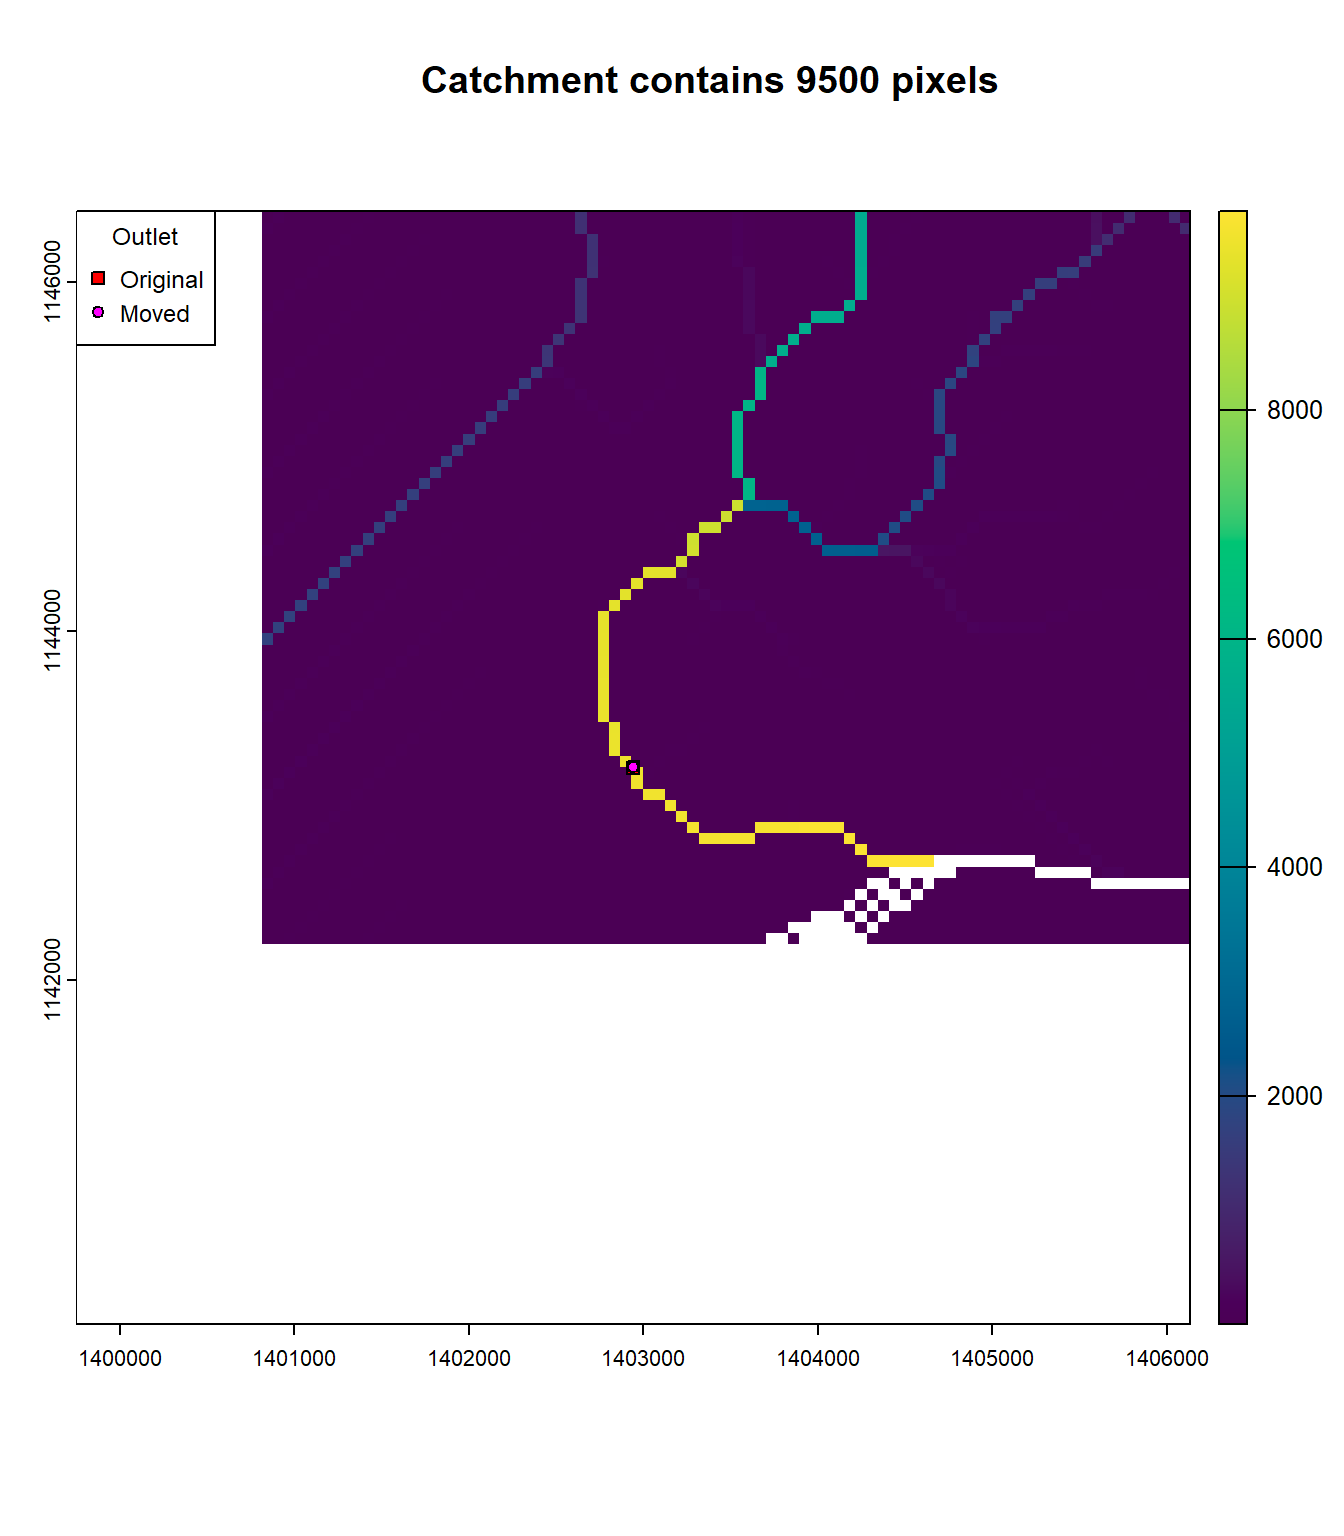
\includegraphics{Illustrating_eDITH_files/figure-latex/unnamed-chunk-26-1.pdf}

\begin{verbatim}
#> Creation of river object...
#> Creation of river object... 100.0%
#> extract_river has finished.
#> Time for DEM download: 1.5 s
#> Time for TauDEM processing: 1.4 s
#> Time for creation of river object: 0.1 s
\end{verbatim}

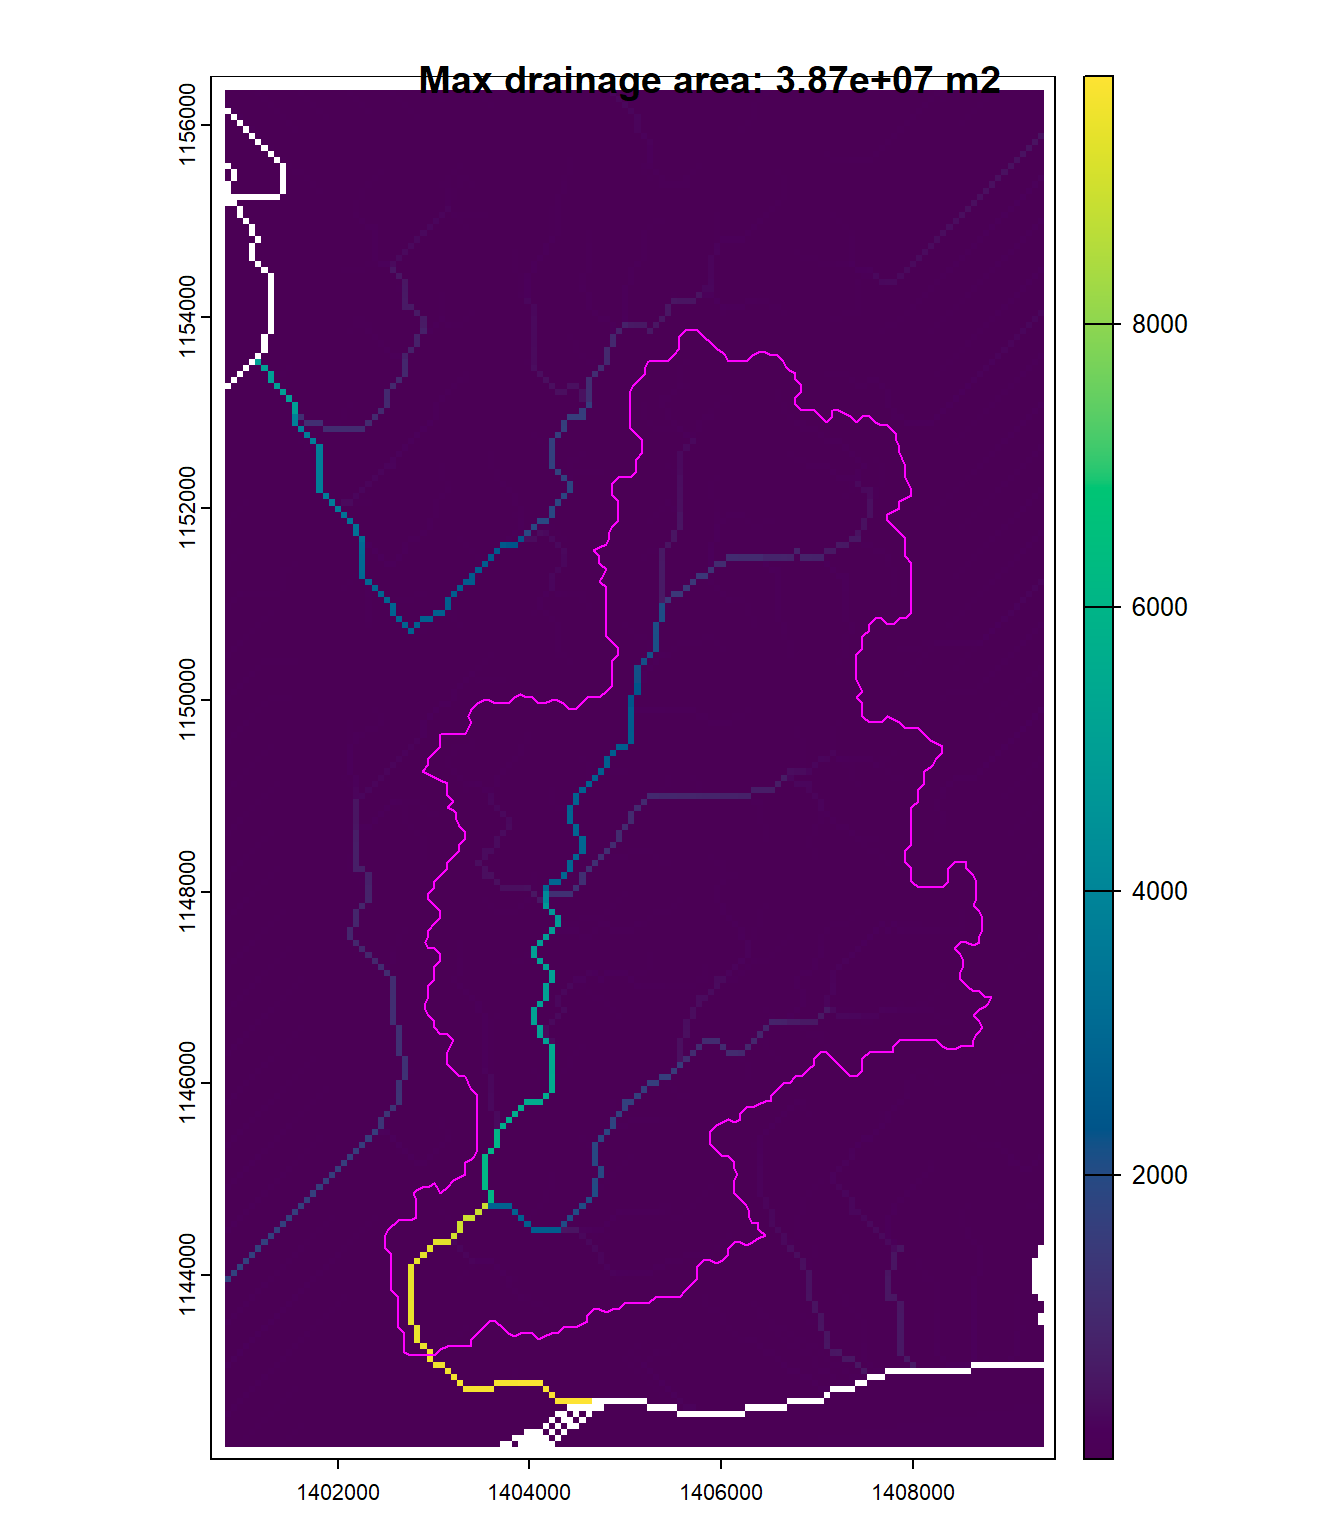
\includegraphics{Illustrating_eDITH_files/figure-latex/unnamed-chunk-26-2.pdf}

\begin{Shaded}
\begin{Highlighting}[]
\CommentTok{\# aggregate river}
\NormalTok{Koide }\OtherTok{\textless{}{-}}\NormalTok{ rivnet}\SpecialCharTok{::}\FunctionTok{aggregate\_river}\NormalTok{(Koide, }\AttributeTok{thrA=}\NormalTok{riverData}\SpecialCharTok{$}\NormalTok{thrA[}\DecValTok{2}\NormalTok{],}
                                 \AttributeTok{maxReachLength=}\DecValTok{1000}\NormalTok{,}
                                 \AttributeTok{equalizeLengths=}\ConstantTok{TRUE}\NormalTok{)}
\CommentTok{\# create data frame with hydrological variables}
\NormalTok{hd }\OtherTok{\textless{}{-}} \FunctionTok{data.frame}\NormalTok{(}\AttributeTok{data=}\FunctionTok{c}\NormalTok{(riverData}\SpecialCharTok{$}\NormalTok{Q.outlet[}\DecValTok{2}\NormalTok{], riverData}\SpecialCharTok{$}\NormalTok{w.outlet[}\DecValTok{2}\NormalTok{]),}
                 \AttributeTok{type=}\FunctionTok{c}\NormalTok{(}\StringTok{"Q"}\NormalTok{, }\StringTok{"w"}\NormalTok{),}
                 \AttributeTok{node=}\FunctionTok{c}\NormalTok{(}\DecValTok{1}\NormalTok{,}\DecValTok{1}\NormalTok{)}\SpecialCharTok{*}\NormalTok{Koide}\SpecialCharTok{$}\NormalTok{AG}\SpecialCharTok{$}\NormalTok{outlet)}
\CommentTok{\# extrapolate hydrological variables}
\NormalTok{Koide }\OtherTok{\textless{}{-}} \FunctionTok{hydro\_river}\NormalTok{(hd, Koide)}
\end{Highlighting}
\end{Shaded}

\hypertarget{pinpoiting-sampling-sites-to-the-river-reaches-1}{%
\subsection{Pinpoiting sampling sites to the river reaches}\label{pinpoiting-sampling-sites-to-the-river-reaches-1}}

In this case, all sampling sites are attributed to the correct reach by \texttt{locate\_site}.

\begin{Shaded}
\begin{Highlighting}[]
\NormalTok{samplingSitesKoide }\OtherTok{\textless{}{-}} \FunctionTok{read.csv}\NormalTok{(}\AttributeTok{file=}\StringTok{"../data/samplingSitesKoide.csv"}\NormalTok{)}

\NormalTok{AGnode }\OtherTok{\textless{}{-}} \FunctionTok{numeric}\NormalTok{(}\FunctionTok{length}\NormalTok{(samplingSitesKoide}\SpecialCharTok{$}\NormalTok{X))}
\ControlFlowTok{for}\NormalTok{ (j }\ControlFlowTok{in} \DecValTok{1}\SpecialCharTok{:} \FunctionTok{length}\NormalTok{(samplingSitesKoide}\SpecialCharTok{$}\NormalTok{X))\{}
\NormalTok{  tmp }\OtherTok{\textless{}{-}}\NormalTok{ rivnet}\SpecialCharTok{::}\FunctionTok{locate\_site}\NormalTok{(samplingSitesKoide}\SpecialCharTok{$}\NormalTok{X[j], }
\NormalTok{                             samplingSitesKoide}\SpecialCharTok{$}\NormalTok{Y[j], }
\NormalTok{                             Koide, }
                             \AttributeTok{showPlot =}\NormalTok{ F)}
\NormalTok{  AGnode[j] }\OtherTok{\textless{}{-}}\NormalTok{ tmp}\SpecialCharTok{$}\NormalTok{AGnode}
\NormalTok{\}}
\NormalTok{samplingSitesKoide[[}\StringTok{"AGnode"}\NormalTok{]] }\OtherTok{\textless{}{-}}\NormalTok{ AGnode}
\end{Highlighting}
\end{Shaded}

\hypertarget{apply-the-edith-model-1}{%
\subsection{Apply the eDITH model}\label{apply-the-edith-model-1}}

\hypertarget{initialization-2}{%
\subsubsection{Initialization}\label{initialization-2}}

Read counts are contained in \texttt{siteSpeciesTableKoide.csv}. The following are the species with at least \texttt{thr\_species} detections:

\begin{Shaded}
\begin{Highlighting}[]
 \CommentTok{\# read species{-}by{-}site table}
\NormalTok{  SST}\SpecialCharTok{$}\NormalTok{Koide }\OtherTok{\textless{}{-}} \FunctionTok{read.csv}\NormalTok{(}\StringTok{"../data/siteSpeciesTableKoide.csv"}\NormalTok{)}
\NormalTok{  SST}\SpecialCharTok{$}\NormalTok{Koide[}\FunctionTok{is.na}\NormalTok{(SST}\SpecialCharTok{$}\NormalTok{Koide)] }\OtherTok{\textless{}{-}} \DecValTok{0} 
\NormalTok{  speciesID}\SpecialCharTok{$}\NormalTok{Koide }\OtherTok{\textless{}{-}} \FunctionTok{which}\NormalTok{(}\FunctionTok{rowSums}\NormalTok{(SST}\SpecialCharTok{$}\NormalTok{Koide[,}\SpecialCharTok{{-}}\DecValTok{1}\NormalTok{]}\SpecialCharTok{!=}\DecValTok{0}\NormalTok{) }\SpecialCharTok{\textgreater{}=}\NormalTok{ thr\_species) }
\NormalTok{  SST}\SpecialCharTok{$}\NormalTok{Koide[speciesID}\SpecialCharTok{$}\NormalTok{Koide,}\DecValTok{1}\NormalTok{]}
\CommentTok{\#\textgreater{}  [1] "Anguilla japonica"                      }
\CommentTok{\#\textgreater{}  [2] "Carassius spp."                         }
\CommentTok{\#\textgreater{}  [3] "Cyprinus carpio"                        }
\CommentTok{\#\textgreater{}  [4] "Hemibarbus spp."                        }
\CommentTok{\#\textgreater{}  [5] "Pseudogobio esocinus"                   }
\CommentTok{\#\textgreater{}  [6] "Pseudorasbora parva"                    }
\CommentTok{\#\textgreater{}  [7] "Rhynchocypris lagowskii steindach{-} neri"}
\CommentTok{\#\textgreater{}  [8] "Tribolodon brandtii maruta"             }
\CommentTok{\#\textgreater{}  [9] "Tribolodon hakonensis"                  }
\CommentTok{\#\textgreater{} [10] "Opsariichthys platypus"                 }
\CommentTok{\#\textgreater{} [11] "Misgurnus anguillicaudatus"             }
\CommentTok{\#\textgreater{} [12] "Paramisgurnus dabryanus"                }
\CommentTok{\#\textgreater{} [13] "Silurus asotus"                         }
\CommentTok{\#\textgreater{} [14] "Plecoglossus altivelis"                 }
\CommentTok{\#\textgreater{} [15] "Mugil cephalus"                         }
\CommentTok{\#\textgreater{} [16] "Oryzias latipes"                        }
\CommentTok{\#\textgreater{} [17] "Lateolabrax japonicus"                  }
\CommentTok{\#\textgreater{} [18] "Eleotris oxycephala"                    }
\CommentTok{\#\textgreater{} [19] "Gymnogobius petschiliensis"             }
\CommentTok{\#\textgreater{} [20] "Rhinogobius giurinus"                   }
\CommentTok{\#\textgreater{} [21] "Rhinogobius spp."                       }
\CommentTok{\#\textgreater{} [22] "Tridentiger spp."                       }
\CommentTok{\#\textgreater{} [23] "Channa argus"}
\end{Highlighting}
\end{Shaded}

\begin{Shaded}
\begin{Highlighting}[]
  \CommentTok{\# initialize variables for export}
\NormalTok{  probDet}\SpecialCharTok{$}\NormalTok{Koide }\OtherTok{\textless{}{-}} \FunctionTok{data.frame}\NormalTok{(}\FunctionTok{matrix}\NormalTok{(}\DecValTok{0}\NormalTok{,Koide}\SpecialCharTok{$}\NormalTok{AG}\SpecialCharTok{$}\NormalTok{nNodes, }
                                     \FunctionTok{length}\NormalTok{(speciesID}\SpecialCharTok{$}\NormalTok{Koide)))}
  \FunctionTok{names}\NormalTok{(probDet}\SpecialCharTok{$}\NormalTok{Koide) }\OtherTok{\textless{}{-}}\NormalTok{ SST}\SpecialCharTok{$}\NormalTok{Koide[speciesID}\SpecialCharTok{$}\NormalTok{Koide,}\DecValTok{1}\NormalTok{]}

\NormalTok{  signifCovariates}\SpecialCharTok{$}\NormalTok{Koide }\OtherTok{\textless{}{-}} \FunctionTok{data.frame}\NormalTok{(}\FunctionTok{matrix}\NormalTok{(}\DecValTok{0}\NormalTok{,n\_covariates,}
                                              \FunctionTok{length}\NormalTok{(speciesID}\SpecialCharTok{$}\NormalTok{Koide)))}
  \FunctionTok{names}\NormalTok{(signifCovariates}\SpecialCharTok{$}\NormalTok{Koide) }\OtherTok{\textless{}{-}}\NormalTok{ SST}\SpecialCharTok{$}\NormalTok{Koide[speciesID}\SpecialCharTok{$}\NormalTok{Koide,}\DecValTok{1}\NormalTok{]}

  \FunctionTok{row.names}\NormalTok{(signifCovariates}\SpecialCharTok{$}\NormalTok{Koide) }\OtherTok{\textless{}{-}} \FunctionTok{paste0}\NormalTok{(}\StringTok{"beta\_AEM"}\NormalTok{,}\DecValTok{1}\SpecialCharTok{:}\NormalTok{n\_covariates)}
\NormalTok{  gelmanDiag}\SpecialCharTok{$}\NormalTok{Koide }\OtherTok{\textless{}{-}} \FunctionTok{data.frame}\NormalTok{(}\FunctionTok{matrix}\NormalTok{(}\DecValTok{0}\NormalTok{,n\_covariates}\SpecialCharTok{+}\DecValTok{3}\NormalTok{,}
                                        \FunctionTok{length}\NormalTok{(speciesID}\SpecialCharTok{$}\NormalTok{Koide)))}

  \FunctionTok{names}\NormalTok{(gelmanDiag}\SpecialCharTok{$}\NormalTok{Koide) }\OtherTok{\textless{}{-}}\NormalTok{ SST}\SpecialCharTok{$}\NormalTok{Koide[speciesID}\SpecialCharTok{$}\NormalTok{Koide,}\DecValTok{1}\NormalTok{]}
  \FunctionTok{row.names}\NormalTok{(gelmanDiag}\SpecialCharTok{$}\NormalTok{Koide) }\OtherTok{\textless{}{-}} \FunctionTok{c}\NormalTok{(}\StringTok{"tau"}\NormalTok{,}\StringTok{"log\_p0"}\NormalTok{,}
                                   \FunctionTok{paste0}\NormalTok{(}\StringTok{"beta\_AEM"}\NormalTok{,}\DecValTok{1}\SpecialCharTok{:}\NormalTok{n\_covariates),}\StringTok{"omega"}\NormalTok{)}
\end{Highlighting}
\end{Shaded}

\hypertarget{run-edith-for-all-species-1}{%
\subsubsection{Run eDITH for all species}\label{run-edith-for-all-species-1}}

\begin{Shaded}
\begin{Highlighting}[]
\ControlFlowTok{for}\NormalTok{ (iS }\ControlFlowTok{in} \DecValTok{1}\SpecialCharTok{:}\FunctionTok{length}\NormalTok{(speciesID}\SpecialCharTok{$}\NormalTok{Koide))\{ }\CommentTok{\# loop over species}
\NormalTok{  indSp }\OtherTok{\textless{}{-}}\NormalTok{ speciesID}\SpecialCharTok{$}\NormalTok{Koide[iS]}
\NormalTok{  nam }\OtherTok{\textless{}{-}}\NormalTok{ SST}\SpecialCharTok{$}\NormalTok{Koide[indSp,}\DecValTok{1}\NormalTok{]}
\NormalTok{  fnam }\OtherTok{\textless{}{-}} \FunctionTok{paste0}\NormalTok{(}\StringTok{\textquotesingle{}../resultsKoide/\textquotesingle{}}\NormalTok{,nam,}\StringTok{\textquotesingle{}.rda\textquotesingle{}}\NormalTok{)}
  
  \ControlFlowTok{if}\NormalTok{(}\SpecialCharTok{!}\FunctionTok{file.exists}\NormalTok{(fnam))\{ }\CommentTok{\# if eDITH results were already generated, skip}
\NormalTok{  values }\OtherTok{\textless{}{-}} \FunctionTok{as.numeric}\NormalTok{(SST}\SpecialCharTok{$}\NormalTok{Koide[indSp,}\SpecialCharTok{{-}}\DecValTok{1}\NormalTok{])}
\NormalTok{  data }\OtherTok{\textless{}{-}} \FunctionTok{data.frame}\NormalTok{(}\AttributeTok{ID=}\NormalTok{samplingSitesKoide}\SpecialCharTok{$}\NormalTok{AGnode, }\AttributeTok{values=}\NormalTok{values) }
  \CommentTok{\# for the species at hand}
  \CommentTok{\# run eDITH model via BayesianTools}
\NormalTok{  out }\OtherTok{\textless{}{-}} \FunctionTok{run\_eDITH\_BT}\NormalTok{(data, Koide, }\AttributeTok{ll.type=}\StringTok{"nbinom"}\NormalTok{,}
                      \AttributeTok{n.AEM=}\NormalTok{n\_covariates, }\AttributeTok{par.AEM=}\FunctionTok{list}\NormalTok{(}\AttributeTok{weight=}\StringTok{"exponential"}\NormalTok{),}
                      \AttributeTok{verbose=}\NormalTok{T)}
  \CommentTok{\# evaluate quantiles from posterior distribution}
\NormalTok{  out }\OtherTok{\textless{}{-}} \FunctionTok{eval\_posterior\_eDITH}\NormalTok{(out, Koide, }\AttributeTok{quant=}\FunctionTok{c}\NormalTok{(}\FloatTok{0.025}\NormalTok{,}\FloatTok{0.5}\NormalTok{, }\FloatTok{0.975}\NormalTok{))}
  \CommentTok{\# run posterior predictive simulations}
\NormalTok{  pps }\OtherTok{\textless{}{-}} \FunctionTok{posterior\_pred\_sim\_eDITH}\NormalTok{(out, Koide)}
  
\NormalTok{  \} }\ControlFlowTok{else}\NormalTok{ \{}\FunctionTok{load}\NormalTok{(fnam)\} }\CommentTok{\# if results already generated, load them}
  
  \CommentTok{\# store posterior median detection probability, }
  \CommentTok{\#    Gelman diagnostics and significance of covariates}
\NormalTok{  probDet}\SpecialCharTok{$}\NormalTok{Koide[,iS] }\OtherTok{\textless{}{-}}\NormalTok{ out}\SpecialCharTok{$}\NormalTok{probDetection\_quantile[}\DecValTok{2}\NormalTok{,]}
\NormalTok{  gelmanDiag}\SpecialCharTok{$}\NormalTok{Koide[,iS] }\OtherTok{\textless{}{-}}\NormalTok{ out}\SpecialCharTok{$}\NormalTok{gD}\SpecialCharTok{$}\NormalTok{psrf[,}\DecValTok{1}\NormalTok{]}
  \ControlFlowTok{for}\NormalTok{ (j }\ControlFlowTok{in} \DecValTok{1}\SpecialCharTok{:}\FunctionTok{length}\NormalTok{(out}\SpecialCharTok{$}\NormalTok{covariates))\{}
    \ControlFlowTok{if}\NormalTok{ (out}\SpecialCharTok{$}\NormalTok{cI[}\DecValTok{1}\NormalTok{,j}\SpecialCharTok{+}\DecValTok{2}\NormalTok{]}\SpecialCharTok{\textgreater{}}\DecValTok{0}\NormalTok{) signifCovariates}\SpecialCharTok{$}\NormalTok{Koide[j,iS] }\OtherTok{\textless{}{-}} \DecValTok{1}
    \ControlFlowTok{if}\NormalTok{ (out}\SpecialCharTok{$}\NormalTok{cI[}\DecValTok{2}\NormalTok{,j}\SpecialCharTok{+}\DecValTok{2}\NormalTok{]}\SpecialCharTok{\textless{}}\DecValTok{0}\NormalTok{) signifCovariates}\SpecialCharTok{$}\NormalTok{Koide[j,iS] }\OtherTok{\textless{}{-}} \SpecialCharTok{{-}}\DecValTok{1}
\NormalTok{  \}}
\NormalTok{\}}
\end{Highlighting}
\end{Shaded}

\hypertarget{displaying-species-richness}{%
\section{Displaying species richness}\label{displaying-species-richness}}

Finally, species richness predicted by eDITH can be computed by stacking up presence/absence predictions for all species contained in the datasets; in turn, these are derived by using a threhsold of 0.5 on the posterior median detection probability. We visually compare the predicted species richness with the observed one at the sampling sites, which we show as colored points in the river map. We also display the modelled detection probability for one characteristic species for each case study, together with the respective observed read counts. This figure corresponds to Fig. 4 shown in the manuscript.

\begin{Shaded}
\begin{Highlighting}[]
\NormalTok{sp\_name }\OtherTok{\textless{}{-}} \FunctionTok{c}\NormalTok{(}\StringTok{"Cottus bairdii"}\NormalTok{,}\StringTok{"Eleotris oxycephala"}\NormalTok{) }
\NormalTok{deu }\OtherTok{\textless{}{-}} \FunctionTok{colorRampPalette}\NormalTok{(}\FunctionTok{c}\NormalTok{(}\StringTok{"yellow"}\NormalTok{,}\StringTok{"red"}\NormalTok{,}\StringTok{"black"}\NormalTok{))}
\NormalTok{north\_length }\OtherTok{\textless{}{-}} \FunctionTok{c}\NormalTok{(}\DecValTok{5000}\NormalTok{,}\DecValTok{1000}\NormalTok{)}
\FunctionTok{par}\NormalTok{(}\AttributeTok{mfrow=}\FunctionTok{c}\NormalTok{(}\DecValTok{2}\NormalTok{,}\DecValTok{2}\NormalTok{), }\AttributeTok{oma=}\FunctionTok{c}\NormalTok{(}\DecValTok{3}\NormalTok{,}\DecValTok{0}\NormalTok{,}\DecValTok{0}\NormalTok{,}\DecValTok{0}\NormalTok{))}
\ControlFlowTok{for}\NormalTok{ (i }\ControlFlowTok{in} \DecValTok{1}\SpecialCharTok{:}\FunctionTok{length}\NormalTok{(riverData}\SpecialCharTok{$}\NormalTok{river)) \{}
\NormalTok{  ID }\OtherTok{\textless{}{-}}\NormalTok{ riverData}\SpecialCharTok{$}\NormalTok{river[i]}
  \FunctionTok{eval}\NormalTok{(}\FunctionTok{parse}\NormalTok{(}\AttributeTok{text=}\FunctionTok{paste0}\NormalTok{(}\StringTok{\textquotesingle{}river \textless{}{-} \textquotesingle{}}\NormalTok{,ID)))}
  \FunctionTok{eval}\NormalTok{(}\FunctionTok{parse}\NormalTok{(}\AttributeTok{text=}\FunctionTok{paste0}\NormalTok{(}\StringTok{\textquotesingle{}samplingSites \textless{}{-} samplingSites\textquotesingle{}}\NormalTok{,ID)))}
  \FunctionTok{plot}\NormalTok{(probDet[[i]][[sp\_name[i]]],  river,}
       \AttributeTok{colPalette=}\FunctionTok{hcl.colors}\NormalTok{(}\DecValTok{1000}\NormalTok{, }\StringTok{"Reds 3"}\NormalTok{, }\AttributeTok{rev=}\NormalTok{T), }\AttributeTok{colLevels =} \FunctionTok{c}\NormalTok{(}\DecValTok{0}\NormalTok{,}\DecValTok{1}\NormalTok{),}
       \AttributeTok{args\_imagePlot=}\FunctionTok{list}\NormalTok{(}\AttributeTok{legend.lab=}\StringTok{"Posterior median detection probability"}\NormalTok{))}
\NormalTok{  values }\OtherTok{\textless{}{-}}\NormalTok{ SST[[i]][}\FunctionTok{which}\NormalTok{(SST[[i]][,}\DecValTok{1}\NormalTok{]}\SpecialCharTok{==}\NormalTok{sp\_name[i]),}\SpecialCharTok{{-}}\DecValTok{1}\NormalTok{]}
  \FunctionTok{points\_colorscale}\NormalTok{(samplingSites}\SpecialCharTok{$}\NormalTok{X, samplingSites}\SpecialCharTok{$}\NormalTok{Y, }\FunctionTok{log10}\NormalTok{(}\FunctionTok{as.numeric}\NormalTok{(values)),}
                    \AttributeTok{cex=}\DecValTok{1}\NormalTok{, }\AttributeTok{force.range =} \ConstantTok{FALSE}\NormalTok{,}
                    \AttributeTok{bg.palette=}\FunctionTok{hcl.colors}\NormalTok{(}\DecValTok{1000}\NormalTok{, }\StringTok{"Blues 3"}\NormalTok{, }\AttributeTok{rev=}\NormalTok{T),}
                    \AttributeTok{bg.range=}\FunctionTok{c}\NormalTok{(}\DecValTok{1}\NormalTok{,}\DecValTok{5}\NormalTok{),}
                    \AttributeTok{horizontal=}\NormalTok{T, }\AttributeTok{legend.lab =} \StringTok{"Observed read counts (log 10)"}\NormalTok{)}
  \FunctionTok{title}\NormalTok{(sp\_name[i])}

  \FunctionTok{plot}\NormalTok{(}\FunctionTok{rowSums}\NormalTok{(probDet[[i]]}\SpecialCharTok{\textgreater{}}\FloatTok{0.5}\NormalTok{), river, }\AttributeTok{addLegend=}\NormalTok{F, }\AttributeTok{max\_lwd=}\DecValTok{3}\NormalTok{, }
       \AttributeTok{colLevels=}\FunctionTok{c}\NormalTok{(}\DecValTok{0}\NormalTok{,}\DecValTok{25}\NormalTok{))}
\NormalTok{  terra}\SpecialCharTok{::}\FunctionTok{sbar}\NormalTok{(}\AttributeTok{d =} \DecValTok{1000}\NormalTok{,}
              \AttributeTok{xy =} \FunctionTok{c}\NormalTok{(}\FunctionTok{min}\NormalTok{(river}\SpecialCharTok{$}\NormalTok{FD}\SpecialCharTok{$}\NormalTok{X)}\SpecialCharTok{+}\FloatTok{0.05}\SpecialCharTok{*}\NormalTok{(}\FunctionTok{max}\NormalTok{(river}\SpecialCharTok{$}\NormalTok{FD}\SpecialCharTok{$}\NormalTok{X)}\SpecialCharTok{{-}}\FunctionTok{min}\NormalTok{(river}\SpecialCharTok{$}\NormalTok{FD}\SpecialCharTok{$}\NormalTok{X)),}
                     \FunctionTok{min}\NormalTok{(river}\SpecialCharTok{$}\NormalTok{FD}\SpecialCharTok{$}\NormalTok{Y)}\SpecialCharTok{+}\FloatTok{0.7}\SpecialCharTok{*}\NormalTok{(}\FunctionTok{max}\NormalTok{(river}\SpecialCharTok{$}\NormalTok{FD}\SpecialCharTok{$}\NormalTok{Y)}\SpecialCharTok{{-}}\FunctionTok{min}\NormalTok{(river}\SpecialCharTok{$}\NormalTok{FD}\SpecialCharTok{$}\NormalTok{Y))))}
\NormalTok{  terra}\SpecialCharTok{::}\FunctionTok{north}\NormalTok{(}\AttributeTok{d =}\NormalTok{ north\_length[i],}
               \AttributeTok{xy =} \FunctionTok{c}\NormalTok{(}\FunctionTok{min}\NormalTok{(river}\SpecialCharTok{$}\NormalTok{FD}\SpecialCharTok{$}\NormalTok{X)}\SpecialCharTok{+}\FloatTok{0.05}\SpecialCharTok{*}\NormalTok{(}\FunctionTok{max}\NormalTok{(river}\SpecialCharTok{$}\NormalTok{FD}\SpecialCharTok{$}\NormalTok{X)}\SpecialCharTok{{-}}\FunctionTok{min}\NormalTok{(river}\SpecialCharTok{$}\NormalTok{FD}\SpecialCharTok{$}\NormalTok{X)),}
                      \FunctionTok{min}\NormalTok{(river}\SpecialCharTok{$}\NormalTok{FD}\SpecialCharTok{$}\NormalTok{Y)}\SpecialCharTok{+}\FloatTok{0.9}\SpecialCharTok{*}\NormalTok{(}\FunctionTok{max}\NormalTok{(river}\SpecialCharTok{$}\NormalTok{FD}\SpecialCharTok{$}\NormalTok{Y)}\SpecialCharTok{{-}}\FunctionTok{min}\NormalTok{(river}\SpecialCharTok{$}\NormalTok{FD}\SpecialCharTok{$}\NormalTok{Y))))}
\NormalTok{  rivnet}\SpecialCharTok{::}\FunctionTok{points\_colorscale}\NormalTok{(samplingSites}\SpecialCharTok{$}\NormalTok{X, samplingSites}\SpecialCharTok{$}\NormalTok{Y, }
                            \FunctionTok{colSums}\NormalTok{(SST[[i]][speciesID[[i]],}\SpecialCharTok{{-}}\DecValTok{1}\NormalTok{]}\SpecialCharTok{\textgreater{}}\DecValTok{0}\NormalTok{),}
                    \AttributeTok{bg.palette =} \FunctionTok{deu}\NormalTok{(}\DecValTok{1000}\NormalTok{),}\AttributeTok{bg.range=}\FunctionTok{c}\NormalTok{(}\DecValTok{0}\NormalTok{,}\DecValTok{25}\NormalTok{),}
                    \AttributeTok{cex=}\DecValTok{1}\NormalTok{, }\AttributeTok{horizontal =}\NormalTok{ T, }\AttributeTok{legend.lab =} \StringTok{"Species richness"}\NormalTok{)}
\NormalTok{\}}
\end{Highlighting}
\end{Shaded}

\includegraphics{Illustrating_eDITH_files/figure-latex/unnamed-chunk-31-1.pdf}

Note the use of \texttt{sbar} and \texttt{north} from the \texttt{terra} package in order to display the scale bar and north arrow, respectively. For both functions, argument \texttt{xy} is mandatory (see also documentation of \texttt{rivnet}'s \texttt{plot}). We here specify \texttt{xy} as a function of the range of the river's coordinates.

\hypertarget{references}{%
\section*{References}\label{references}}
\addcontentsline{toc}{section}{References}

\hypertarget{refs}{}
\begin{CSLReferences}{1}{0}
\leavevmode\vadjust pre{\hypertarget{ref-balasingham2018}{}}%
Balasingham, K. D., R. P. Walter, N. E. Mandra, and D. D. Heath. 2018. {``Environmental DNA Detection of Rare and Invasive Fish Species in Two Great Lakes Tributaries.''} \emph{Molecular Ecology}. \url{https://doi.org/10.1111/mec.14395}.

\leavevmode\vadjust pre{\hypertarget{ref-blanchet2008}{}}%
Blanchet, F. G., P. Legendre, and D. Borcard. 2008. {``Modelling Directional Spatial Processes in Ecological Data.''} \emph{Ecological Modelling}. \url{https://doi.org/10.1016/j.ecolmodel.2008.04.001}.

\leavevmode\vadjust pre{\hypertarget{ref-carraro2022}{}}%
Carraro, L., and F. Altermatt. 2022. {``Optimal Channel Networks Accurately Model Ecologically-Relevant Geomorphological Features of Branching River Networks.''} \emph{Communications Earth and Environment}. \url{https://doi.org/10.1038/s43247-022-00454-1}.

\leavevmode\vadjust pre{\hypertarget{ref-sakata2021}{}}%
Sakata, M. K., T. Watanabe, N. Maki, K. Ikeda, T. Kosuge, H. Okada, H. Yamanaka, T. Sado, M. Miya, and T. Minamoto. 2021. {``Determining an Effective Sampling Method for eDNA Metabarcoding; a Case Study for Fish Biodiversity Monitoring in a Small, Natural River.''} \emph{Limnology}. \url{https://doi.org/10.1007/s10201-020-00645-9}.

\end{CSLReferences}

\end{document}
